% !TEX TS-program = xelatex
% !TEX encoding = UTF-8 Unicode
% !Mode:: "TeX:UTF-8"
\documentclass[bachelor,nocolorlinks, printoneside]{seuthesis} % 本科
% \documentclass[master]{seuthesis} % 硕士
% \documentclass[doctor]{seuthesis} % 博士
% \documentclass[engineering]{seuthesis} % 工程硕士
\usepackage{ctex}
\usepackage{CJK,CJKnumb}
\usepackage{amsmath}
\usepackage{amsfonts} 
\usepackage{bm} 
\usepackage{algorithm}
\usepackage{algorithmicx}
\usepackage{algpseudocode}
\usepackage{subfigure}
\usepackage{latexsym}
\usepackage{amsthm}
\usepackage{enumitem}
\usepackage{multirow}
\usepackage[section]{placeins}
\usepackage{float}
\usepackage{indentfirst} 
\usepackage{booktabs}
\usepackage{enumerate}
\usepackage{amssymb}

\floatname{algorithm}{算法}
\renewcommand{\algorithmicrequire}{\textbf{输入:}}
\renewcommand{\algorithmicensure}{\textbf{输出:}}
 % 这里是导言区

\begin{document}

\categorynumber{000} % 分类采用《中国图书资料分类法》
\UDC{000}            %《国际十进分类法UDC》的类号
\secretlevel{公开}    %学位论文密级分为"公开"、"内部"、"秘密"和"机密"四种
\studentid{04015124}   %学号要完整,前面的零不能省略。

\title{大规模MIMO的检测与估计}{}{Detection and Estimation of Massive MIMO System}{subtitle}
\author{郑奕飞}{Yifei Zheng}
\advisor{孙晨}{讲师}{Chen Sun}{Prof.}
\coadvisor{王闻今}{教授}{Wenjin Wang}{Associate Prof.} % 没有

% \degree{工学硕士} % 详细学位名称
\major[12em]{信息工程}
\defenddate{答辩日期}
\authorizedate{学位授予日期}
\department{信息科学与工程学院}{department name}
\duration{2019年1月—2019年6月}
\address{无线谷1405室}
\maketitle

\begin{abstract}{关键词}
待定
\end{abstract}

\begin{englishabstract}{KEY Word}
待定
\end{englishabstract}

\tableofcontents


\begin{Main} % 开始正文

\chapter{绪论}
\section{研究背景}
由于智能设备,移动设备广泛使用以及实现M2M通信的目标,全球移动通信网络所需要传输的数据量猛增。并且目前的设计受制于通信频谱的不足。为了解决通信的数据量猛增以及低损的频谱波段的不足的问题,所以考虑使用大规模多输入多输出传输技术(LS-MIMO)。并且第五代通信系统也致力于研究大规模MIMO的技术,所以5G相关的基础技术很多也是和大规模MIMO相关的。

并且目前的毫米波发展导致传输相同的距离需要更高的功率或者比3G/4G更多的基站,此时我们也需要大规模MIMO的发展来建立适合小蜂窝的网络结构。

大规模MIMO检测是大规模MIMO技术的一部分,并且是基础功能。大规模MIMO检测目前主要使用的是最小均方误差估计(MMSE检测)技术,其很大的问题是MMSE检测的复杂度。一般MMSE对于大规模MIMO系统复杂度是相当大的,计算复杂度过大带来的问题是对于硬件的计算能力和计算时延有一定的要求。
选题的研究方向主要就是研究低复杂度的检测算法,并且通过建立大规模MIMO空间信道模型验证其正确性。

大规模MIMO系统影响接收信号强度主要的原因是多径传输,多普勒影响,空间特性的影响。多径的影响主要是发送端和接收端之间的有许多不同的传输路径,多普勒影响主要是移动的发送端或者接收端带来的频率偏移,大规模MIMO天线带来的波束指向性会带了空间特性。而与传统的MIMO不同的是大规模MIMO有一些特别的性质,包括更有利的发射状态,发射角特性,球形波阵面假设和空间不稳定特征。目前的大规模MIMO信道测量方式主要是利用宽带高同步率的收发机,进行大量的数据传输得到信道参数。并且针对不同情况进行不同的天线设置。目前的信道测试基本上以6GHz以下的频带进行测试,从而验证了大规模MIMO的特别性质。而信道建模的主要分为数据模型和确定性模型。数据模型主要分为基于相关的随机模型和基于几何的随机模型,对于大规模MIMO基于几何的随机模型要更适合一些。而未来大规模MIMO信道建模的研究方向要考虑之前提到的大规模MIMO相对于传统MIMO的特性,并且需要结合第五代移动通信采用的核心技术。

\section{大规模MIMO检测与估计}
在过去五十年对于MIMO系统的检测估计做过很多研究。大规模MIMO的主要影响传输效果的原因是共通道干扰(CCI),而共通道干扰在MIMO中主要体现在符号间干扰(ISI),通道间干扰(ICI),天线间干扰(IAI),多用户干扰(MUI),多接入干扰(MAI),多流干扰(MSI)等等。而需要大规模MIMO检测的主要原因是输入信道不是相互正交,输出就会有相互干扰的情况。而应用模型主要有三种,单用户多天线MIMO的模型(singer-user SDM-MIMO),多用户用户单天线的MIMO模型,多用户多天线的MIMO模型。同时目前考虑了多种不同的大规模MIMO系统模型,线性无记忆MIMO系统,离散保留记忆MIMO系统,实数MIMO系统,复数MIMO系统。前面两种模型都包含有时域和频域,后面两种系统讨论的主要是系统实现的优劣。实数MIMO系统具有实数阵规模小,操作自由,复数MIMO系统具有适应多种调制方式,硬件实现简单以及在某些情况下信道容量会比实数MIMO系统要大。

目前用于大规模MIMO检测的算法有很多不同种,大部分都属于最小方差估计,其中包括最适MIMO检测,经典的线性MIMO检测,基于减少干扰的MIMO检测,基于树状搜索的MIMO检测,降维MIMO检测(LR),概率数据互联MIMO检测(PDA),基于半点松弛编程的MIMO检测。最适MIMO检测最先指的是ML接收机,之后几年的研究讨论了ML,MAP等估计算法的最优标准最终线性MMSE接收机确定为最优的接收机,从而也引出了关于MMSE的计算复杂度的问题。线性MIMO接收机又分为匹配滤波接收机,零干扰接收机,MMSE接收机,其他线性接收机。加性干扰去除MIMO接收机是一个非线性的接收机,效果会比线性MIMO接收机要好,而且根据不同的性质可以有很多种变种形式,性能较好的有successive interference cancellation(SIC)接收机,parallel interference cancellation(PIC)接收机,multistage interference cancellation(MIC)接收机,decision-feedback接收机(DFD)。这种接收机主要问题是如果接收信号较大,会出现错误传输的问题,更适合只需要较小信号的用户。基于树状搜索的MIMO接收机是目前研究多天线接收机的流行方向,其主要优势在于在降低接收机计算复杂度的时候可以逼近甚至达到ML接收机的效果。Lattice-Reduction(LR)接收机是基于经典的几何学和群论推导出的lattice定义的MIMO接收机。其一般被用来和其他MIMO算法结合,通过优化MIMO接收机的信道矩阵优化MIMO检测算法。概率数据互联MIMO检测(PDA)MIMO检测,PDA滤波技术是被Bar-Shalom在1975为了研究在干扰严重的环境下测量结果无法定标和结果错误时追踪和监控目标问题提出来的。此方法本来主要是用来研究雷达追踪目标的功能来实现的。SDM接收机同样是为了对抗复杂环境以及降低复杂度并且取得很好的效果而提出的MIMO接收机。

大规模MIMO检测继Marzetta的开创性工作之后,LS-MIMO系统已经成为一个热门的研究课题。然而,在检测方面,一些早期的研究从大系统分析或渐进性能分析的角度探讨了这个问题。LS-MIMO系统的概念可以看作是无线通信和信号处理领域的一种范式转变。在这种大维背景下,MIMO检测问题变得更加具有挑战性和重要性。
在相关文献调查中,在线性信道上低复杂度的影响缓解可以通过使用随机矩阵理论的收敛结果可以解决优化问题。可以使用自由概率理论对MMSE检测器进行优化,使计算复杂度降低。可以用预先算好的信道矩阵和多项式等式对上行接收机进行优化,并且可以获得相近的检测效果。可以利用牛顿迭代法对大规模MIMO接收机进行优化。同时可以利用基于坐标下降的算法对上行大规模MIMO接收机进行优化。

\chapter{大规模MIMO信道模型}
\section{引言}
无线通信系统的性能取决于无线信道环境,无线信道系统学习与研究都需要合适的无线信道作为基础。无线通信信道主要描述的是无线电波从发送端传播到接收端的过程。无线通信的主要问题在于无线电波传播的过程中,无线电波会收到传播路径中物体的反射、衍射、绕射和散射。反射是指无线电波遇到相对于波长来说很大的物体表面时传播方向发生改变的物理现象,衍射是指无线电波遇到狭缝、小孔时偏离原来直线传播的物理现象,绕射是指无线电波绕过障碍物向前传播的物理现象,散射是指无线电波遇到不光滑表面时扩散传播的物理现象。为便于表述,常把对无线电波传播产生反射、衍射、绕射和散射的各类物体,统称为散射体。相应地,各非直射传播路径均称为散射路径。而对这部分传输过程以及其他原因所对信号产生的影响对其进行数学建模,具有其特征的数学模型就可以称为是无线信道。

无线信道的一个特有的特征是衰落,同样也是信道讨论的关键。经过无线信道传播的信号,其幅度随时间和频率变化。信号的衰落分为大尺度衰落和小尺度衰落。大尺度衰落包括与传播距离有关的路径损耗和大障碍物引起的阴影衰落,小尺度衰落是多径信号叠加和移动台移动引起的信号快速起伏变化。一般会将这两个特征分别进行数学建模,根据研究目标不同,对两种衰落的建模细致程度也会不一样。而本文讨论的大规模MIMO信道还会涉及到MIMO天线阵列对信号传输造成的影响和大规模阵列与普通MIMO信道的不同。


\begin{figure}[htbp!]
	\centering 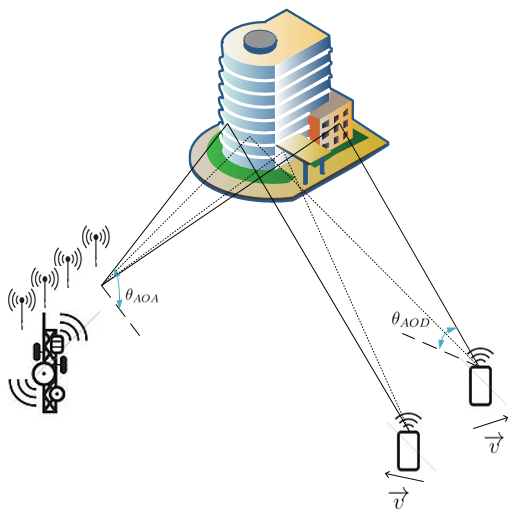
\includegraphics[width=0.45\textwidth]{img/2_1.png} \caption{MIMO场景示意图}
\end{figure}

\section{MIMO信道物理模型}
本论文考虑的是大规模MIMO模型的上行信道,所以本文MIMO模型考虑为固定基站,配备$N_{R}$根天线,移动用户终端配备$N_{T}$根天线,其移动以$\overrightarrow{v}$表示。而城市中信道模型主要考虑的是信号传输在其中的多径情况,信号经过不同的物体表面会出现发射吸收等情况,导致最后到达接收端出现衰落,时延和相位变化。并且考虑到用户终端是移动的,会产生不同径上不同程度上的多普勒频偏。并且MIMO模型与一般的SISO模型不相同的地方在于天线阵列会提供天线阵列带来的发射和接收增益,所以我们可以将信道模型写为如下形式
\begin{equation}\label{key}
h_{n_{R},n_{T},p}(t) = \sum_{q=1}^{Q_{p}}u_{n_{R},p,q}h_{p,q}(t)w_{n_{T},p,q}
\end{equation}
其中,式(2.2)意义是信道多径带来的信道响应,式(2.3)(2.4)意义是天线阵列带来的信道响应
\begin{eqnarray}\label{key}
h_{p,q}(t) = \alpha_{LNA}\beta\alpha_{PA}a_{p,q}e^{j(2\pi 
	(v_{p,q}t-f_{c}\tau_{p,q}-v_{p,q}\tau_{p,q})+\phi_{p,q}
	)} \\
w_{n_{T},p,q} = \mathrm{exp}(-j2\pi \frac{d_{n_{T}}}{\lambda}\sin \theta_{p,q,AOD})\\
u_{n_{R},p,q} = \mathrm{exp}(-j2\pi \frac{d_{n_{R}}}{\lambda}\sin \theta_{p,q,AOA})
\end{eqnarray}
以下主要讨论的是信道小尺度衰落的特征,$ v_{p,q} $为多普勒频移 $ v_{p,q} = \frac{v}{\lambda}\cos\theta_{v,p,q} $ 为用户端移动带来的影响$ \phi_{p,q} $为相位变化。
式(2.2)中$a_{p,q}$为相位信号幅度衰减,$\tau_{p,q}$为传播带来的时延,其中时延拓展一般分为最大时延拓展和均方根时延拓展,最大时延拓展定义为最大时延径和最小时延径的时延差,均方根时延拓展分别定义为
\begin{equation}\label{key}
\sigma_{\tau} = \sqrt{ 
	\frac{
		\sum_{p=1}^{P}(\tau_{p}-\overline{\tau})P(\tau_{p})
	}
	{
		\sum_{p=1}^{P}
		P(\tau_{p})
	}
}
\end{equation}
其中,
\begin{equation}\label{key}
\overline{\tau}=\frac
{\sum^{P}_{p=1}\tau_{p}P(\tau_{p})}
{\sum_{p=1}^{P}P(\tau_{p})}
\end{equation}
通常因为不同径距离不同而带来的通过时间的差异,所以一般时延拓展一般多会考虑时延的统计特性。

用$\beta$来表示大尺度衰落,大尺度衰落一方面指的是接收信号功率随着距离的减少,被称为路径损耗,另一方面指的是接收信号功率由于阴影造成的随机衰减,被称为随机衰落。结合两种主要大尺度衰落,一般为了方便计算可以简单的建模为,单位为分贝
\begin{equation}\label{key}
\beta=10 \log_{10} K-10 \gamma \log_{10} \frac{d}{d_{0}}-\psi_{dB}
\end{equation}
其中,$K$是一个常系数,由天线的固有性质决定。$d_{0}$为天线远场的参考距离,$d$为收发端之间的距离,$\psi_{dB}$是零均值,方差为$\sigma_{\psi_{dB}}$的高斯变量。即$10 \log_{10} K $ 为天线的增益,$ 10 \gamma \log_{10}$ 为路径距离带来的影响,研究表明随着路径的增长,路径损耗趋势成指数级,而一般认为在系统定义的远场距离之外才呈现这样的性质,在远场距离之内的一般不考虑这种建模方式,$\gamma$ 一般是考虑载波的频率和天线高度所得出的,$ \psi_{dB}$ 即为随机衰落,主要是由于阴影衰落的带来的,一般建模为log-normal模型
\begin{equation}\label{key}
p(\psi)=\frac{\xi}{\sqrt{2\pi}\sigma_{\psi_{dB}\psi}}\exp\left({-\frac{(10\log_10 \psi - \mu_\psi)^{2}}{2\sigma_{\psi_{dB}}^{2}}}\right),\quad \psi > 0
\end{equation}
而如上面所述,一般单位设置为dB,则改写为下式,并一般以其的高斯分布表示
\begin{equation}\label{key}
p(\psi)=\frac{1}{\sqrt{2\pi}\sigma_{\psi_{dB}}}\exp\left({-\frac{(\psi_{dB} - \mu_\psi)^{2}}{2\sigma_{\psi_{dB}}^{2}}}\right),\quad \psi > 0
\end{equation}
此外,有些考虑视界传输信道(LOS)会将大尺度建模为自由空间传输路损模型。

式(2.3)(2.4)代表的天线阵列信道响应,其中,$d_{n_{T}}$ 表示第$n_{T}$根发送天线与第一根发射天线的距离,$d_{n_{R}}$ 表示第$n_{R}$根接收天线与第一根接收天线的距离。$\theta_{p,q,AOD}$表示的是第p径的第q个子径的离开角,$\theta_{p,q,AOD}$表示的是第p径的第q个子径的到达角。因为基站侧天线阵列天线间隔会导致天线接收到的数据相位上的不同,导致接收天线具有一定的方向性,同理可以推导至发射端以及发射天线,在这种情况下到达角$\theta_{p,q,AOD}$和离开角$\theta_{p,q,AOD}$会比较重要。

对于式(2.2)代表的多径衰落,在不考虑阵列增益时$h_{n_{R},n_{T},p}(t)$是很多个子径之和,子径可以由服从均匀分布的复数表示,这里的$Q_{p}$是比较大,所以一般将$h_{p}(t)$考虑建模为两种信道模型。一种是不考虑直达径的瑞利衰落信道,这里讲$h_{p}(t)$建模为均值为零,方差为$\sigma_{p}^{2}$的复高斯分布随机变量。同时,因为是经过不同的散射体,各径之间相互独立,对于不同的$p_{1}$和$p_{2}$,$h_{p_{1}}$和$h_{p_{2}}$是统计独立的。另一种是考虑直达径的瑞信衰落信道,即第一个径包括直达径,$h_{1}$建模为均值非零的复高斯随机变量,幅值满足瑞信分布。在MIMO模型中因为需要考虑阵列带来的接收和发送增益,所以还需要考虑信道模型中的阵列向量响应。

P径的信道的矩阵形式如下
\begin{equation}\label{key}
\mathbf{H}_{p}(t) = \left[ \begin{array}{cccc}
h_{1,1,p}(t) & h_{1,2,p}(t) & \ldots & h_{1,N_{T},p}(t) \\
h_{2,1,p}(t) & h_{2,2,p}(t) & \ldots & h_{2,N_{T},p}(t) \\
\vdots & \vdots & \ddots & \vdots \\
h_{N_{R},1,p}(t) & h_{N_{R},2,p}(t) & \ldots & h_{N_{R},N_{T},p}(t)
\end{array} \right] 
\end{equation}
由此,信道矩阵表示为
\begin{equation}\label{key}
\mathbf{H}(t,\tau) = \sum_{p=1}^{P}\mathbf{H}_{p}(t)\delta(\tau-\tau_{p})
\end{equation}
写成矩阵形式为
\begin{equation}\label{key}
\mathbf{H}(t) = \left[ \begin{array}{cccc}
\sum_{p=1}^{P}h_{1,1,p}(t) & \sum_{p=1}^{P}h_{1,2,p}(t) & \ldots & \sum_{p=1}^{P}h_{1,N_{T},p}(t) \\
\sum_{p=1}^{P}h_{2,1,p}(t) & \sum_{p=1}^{P}h_{2,2,p}(t) & \ldots & \sum_{p=1}^{P}h_{2,N_{T},p}(t) \\
\vdots & \vdots & \ddots & \vdots \\
\sum_{p=1}^{P}h_{N_{R},1,p}(t) & \sum_{p=1}^{P}h_{N_{R},2,p}(t) & \ldots & \sum_{p=1}^{P}h_{N_{R},N_{T},p}(t)
\end{array} \right]
\end{equation}

本论文讨论的是窄带信号,但是需要注意的是,在考虑宽带情况下,信道都具有具有时间选择性和频率选择性。除此以外,MIMO信道还具有空域选择性,这一特性会导致MIMO信道矩阵各元素具有相关性。信道的功率角度谱和角度拓展用来表示MIMO信道的空域选择性,以$P(\theta_{AOA})$表示到达角为$\theta_{AOA}$方向上信道幅值的均方值,反映$\theta_{AOA}$方向上的平均接收功率,称为信道的功率角度谱。均方根角度拓展定义为
\begin{equation}\label{key}
\sigma_{\theta_{AOA}}=\sqrt{
	\frac{\int_{-\pi}^{\pi}(\theta_{AOA}-\overline{\theta}_{AOA})P(\theta_{AOA})d\theta_{AOA}}
	{\int_{-\pi}^{\pi}P(\theta_{AOA})d\theta_{AOA}}
}
\end{equation}

\section{MIMO信道统计模型}
以上是信道的物理模型,在处理信道时,为了方便处理,一般会使用物理模型特性推导的统计模型,在使用统计模型时需要明确以下概念。

信道信息分为发送端得到的信道信息(CSIT),接收端得到的信道信息(CSIR)。一般考虑的是接收端得到的信道信息,通过发送导频序列进行信道估计能很容易的得到信道增益信息。在有反馈路径的时候,CSIT由接收端将接收端估计出的信道信息(CSIR)发送回去得到。或者在没有反馈路径的双向通信的系统中,CSIT也可以利用传播的倒数特性得到。当系统收发两端都无法得到信道信息时,需要利用一些特殊的数学模型,例如零平均空间白(ZMSW)模型,ZMSW模型中信道矩阵$\mathbf{H}$中的元素被认为是独立同分布的零均值单位方差循环对称的复高斯变量。或者,其中的元素可以是均值非零或者协方差矩阵。关于CSI的不同假设和$\mathbf{H}$中元素的分布主要反映的是不同的信道容量或者是空时响应的不同方式。

考虑带宽为B,零均值,协方差矩阵为$\sigma^{2}\mathbf{I}_{M_{r}}$的噪声,$\sigma^{2} \triangleq \mathbf{E}[n^{2}_{i}]= N_{0}/2$。并有发射信号
\begin{equation}\label{key}
\sum_{i=1}^{M_{t}}\mathbf{E}[x_{i}x_{i}^{*}] = P
\end{equation}
或者可以写为
\begin{equation}\label{key}
\mathbb{E}[\mathrm{tr}(\mathbf{x}\mathbf{x}^{H})] = P
\end{equation}
则信道矩阵有
\begin{equation}\label{key}
\mathbb{E}[\mathrm{tr}(\mathbf{H}\mathbf{H}^{H})] = N_{R}N_{T}
\end{equation}

发射功率约束$P$将根据$P/\sigma^{2} = \rho$得到SNR$\rho$,同时如果考虑天线能量均匀分布的话有$\mathbb{E}[(\mathbf{x}\mathbf{x}^{H})] = (P/N_{t})I_{N_{t}} $,$\rho$可以用来表示在单通道增益下单根接收天线的平均信噪比SNR。为了简化模型,有时会将噪声功率归一化,此时$\rho$也可以用来表示发射功率。

本论文讨论的是双向通信背景下的基站侧的检测估计,所以认为发送接收双方都有信道信息。从式(2.10)可以得到$\mathbf{H}$是一个$N_{R} \times N_{T}$矩阵。考虑该情况下的联合相关信道
\begin{equation}\label{key}
\mathbf{H} = \mathbf{U}_{r}\tilde{\mathbf{H}}\mathbf{U}_{t}^{H} = \mathbf{U}_{r}(\mathbf{D}+\mathbf{M}\odot \mathbf{H}_{idd})\mathbf{U}_{t}^{H}
\end{equation}
其中$\tilde{\mathbf{H}} = \mathbf{D}+\mathbf{M}\odot \mathbf{H}_{idd}$,$\mathbf{U}_{t}$和$\mathbf{U}_{r}$分别是$N_{T} \times N_{T}$维 和$N_{R} \times N_{R}$维的确定酉矩阵。$\mathbf{D}$是一个$N_{R} \times N_{T}$维每行每列至少有一个非零元素的确定性矩阵,$\mathbf{M}$是一个$N_{R} \times N_{T}$维非负确定矩阵,$\mathbf{H}_{i.i.d.}$是一个$N_{R} \times N_{T}$维零均值独立同分布的矩阵。$\mathbf{H}_{i.i.d.}$并不限于是高斯。但本文在上述条件下考虑的是单位方差的高斯矩阵。由上式(2.15)一般定义
\begin{equation}\label{key}
\bm{\Omega} =\mathbb{E}[\tilde{\mathbf{H}} \odot \tilde{\mathbf{H}}^{*}]
\end{equation}
即
\begin{equation}\label{key}
\bm{\Omega} = \mathbf{D} \odot \mathbf{D} + \mathbf{M} \odot \mathbf{M}
\end{equation}
则有
\begin{eqnarray}\label{key}
\mathbf{D} & = & \mathbb{E}[\tilde{\mathbf{H}}] \\
\left[  \mathbf{M} \right]_{ij} & = & \sqrt{\mathrm{var}(\tilde{[\mathbf{H}]}_{ij})} \nonumber \\
& = & \sqrt{[\bm{\Omega}]_{ij}-[D]_{ij}^{2}}
\end{eqnarray}
即矩阵$\mathbf{D}$和$\mathbf{M}$分别代表了信道的LOS和信道的稀疏元素所以又称$\bm{\Omega} $为特征能量耦合矩阵,可以看出特征能量耦合矩阵$\bm{\Omega}$的各行各列是信号传输过程中发送端和接收端相关矩阵的集合,这些本征值是不可分解的,并且代表了信道的联合相关特征。并且根据上述性质,其可以改写发射功率约束为
\begin{equation}\label{key}
\sum_{i=1}^{N_{R}}\sum_{j=1}^{N_{T}}[\bm{\Omega}]_{ij} = N_{T}N_{R}
\end{equation}
又因为式(2.14),可以将发射和接收端的协方差矩阵写为
\begin{eqnarray}\label{key}
\mathbf{R}_{t}=\mathbb{E}\lbrace \mathbf{H}^{H}\mathbf{H} \rbrace = \mathbf{U}_{t}\bm{\Lambda}_{t}\mathbf{U}_{t}^{H} \\
\mathbf{R}_{r}=\mathbb{E}\lbrace \mathbf{H}\mathbf{H}^{H} \rbrace = \mathbf{U}_{r}\bm{\Lambda}_{t}\mathbf{U}_{r}^{H}
\end{eqnarray}
$\bm{\Lambda}_{t}$和$\bm{\Lambda_{r}}$是对角阵,并有
\begin{eqnarray}\label{key}
[\bm{\Lambda}_{t}]_{ii} & = & \sum_{j=1}^{N_{r}} [\bm{\Omega}]_{ji} 
\end{eqnarray}
由此可以说明$\mathbf{U}_{t}$和$\mathbf{U}_{r}$是发送端和接收端协方差矩阵的特征向量矩阵。这些矩阵元素由天线的特性决定。本论文主要讨论的天线阵列为均匀线阵(ULA),所以特征向量矩阵也可以直接写为离散傅里叶变换矩阵(DFT)。

上面推导的联合概率模型是一个泛式,根据$ \mathbf{D}$和$\mathbf{M}$不同取值,可以分为不同的联合概率模型。例如,当$\mathbf{D}=0,\mathbf{M}$是一个秩为1的矩阵,$\mathbf{H}_{i.i.d.}$有瑞利衰落信道,则上述模型为分离相关Kronecker模型。当令$\mathbf{M}$的秩为随机值,将$\mathbf{U}_t$和$\mathbf{U}_t$固定为DFT矩阵,此时获得的信道模型为均匀线阵天线系统的虚拟信道模型。在这基础上,令$\mathbf{U}_t$和$\mathbf{U}_r$为随机酉矩阵,得到的为Weichselberger模型。本论文考虑的主要是在Weichselberger模型基础上令$ \mathbf{D} = 0 $的UIU模型。

除此之外,还有一种常用MIMO信道统计模型是分离相关信道模型,也称为直积信道模型,一般表示为$ \mathbf{H} = \bm{\Theta}_R^{1/2} \mathbf{H}_{i.i.d.} \bm{\Theta}_T^{1/2}$其一般不考虑信道时变特性,并且联合相关信道模型更加贴近实际,所以本论文不考虑直积信道模型的作用。

\section{大规模MIMO波束域信道模型}
推导波束域信道模型,需要预先分析大规模MIMO的空间信道特征,考虑上文提到的物理信道模型式(2.1)和式(2.2),为了后续化简可以将其改写为矩阵形式并合并一些本论文不作具体建模的变量
\begin{equation}\label{key}
\mathbf{H} = \sum_{p=1}^{P}\beta_p \mathbf{u}_{r,p}\mathbf{w}_{t,p}e^{-j2\pi \tau_{p,k}}
\end{equation}
$\beta_p$表示第p径带来的总体增益其中包括之前提到的发射接收增益以及路径衰落。本论文考虑的是均匀线阵天线阵列,并且天线间隔为半波长,根据式(2.3)和式(2.4)可以将阵列响应写成如下的向量形式
\begin{eqnarray}\label{key}
\mathbf{u}_{r,p}(\theta_{AOA}) = [1,e^{-j\pi \sin \theta_{AOA}},...,e^{-j\pi (N_R-1)}\theta_{AOA}] \\
\mathbf{w}_{t,p}(\theta_{AOD}) = [1,e^{-j\pi \sin \theta_{AOD}},...,e^{-j\pi (N_T-1)}\theta_{AOD}]
\end{eqnarray}

为了将模型变换到波束域,这里需要证明一个定理,在大规模MIMO系统条件下,当基站侧天线数趋于无穷时,有离散傅里叶变换(DFT)可以作为信道的特征矩阵。在天线数趋于无穷时,不同到达角AOA的阵列响应相互独立性质,即到达角的响应集中在一个位置。
\begin{equation}\label{key}
\lim_{N_R \rightarrow \infty}\frac{1}{N_R}<\mathbf{u}(\theta_1),\mathbf{u}(\theta_2)> = \delta(\theta_1 -\theta_2)
\end{equation}

将式(2.10)的信道矩阵重写成向量的集合
\begin{equation}\label{key}
\mathbf{H} = [\mathbf{h}_1,\mathbf{h}_2,...,\mathbf{h}_{N_T}]
\end{equation}
其中,
\begin{equation}\label{key}
\mathbf{h}_m = \sum_{p=1}^{P}\beta_p e^{j\pi (n_r-1) \sin(\theta_{AOA})} \mathbf{w}_{t,p}(\theta_{AOD}) e^{-j2\pi\tau_{p}}
\end{equation}
其左乘DFT矩阵,得到信道DFT之后的矩阵
\begin{equation}\label{key}
\mathbf{H}_{F} = \mathbf{F} \mathbf{H} =[\mathbf{h}_{F,1},\mathbf{h}_{F,1},...,\mathbf{h}_{F,N_T}]
\end{equation}
$\mathbf{F}$为$N_R \times N_R $DFT矩阵,其$(n_r,n_r^{'})$元素为
\begin{equation}\label{key}
[ \mathbf{F} ]_{n_r,n_r^{'}} = \frac{1}{\sqrt{N_R}} e^{-j \frac{2\pi (n_r-1)(n_r^{*}-1)}{\mathbf{N_R}}}
\end{equation}
带入式(2.29)可得
\begin{equation}\label{key}
\mathbf{h}_{F,m} = \sum_{p=1}^{P} \beta_p \left( \sum_{i=0}^{N_R-1} \frac{1}{\sqrt{N_R}} e^{j2\pi i(0.5\sin \theta_{AOA} - \frac{N_R}{n_r-1})} \right) \mathbf{w}_{t,p}(\theta_{AOD}) e^{-j2\pi\tau_{p}}
\end{equation}
根据之前提到的性质式(2.27),当基站侧天线趋于无穷时,式(2.32)可以写成
\begin{eqnarray}\label{key}
\lim_{N_R \rightarrow \infty} \sum_{i=0}^{N_R-1} \frac{1}{\sqrt{N_R}} e^{j2\pi i(0.5 \sin \theta_{AOA} -\frac{n_r-1}{N_R})} = \left \lbrace
\begin{array}{l}
0 \quad 0.5\sin \theta_{AOA} - \frac{n_r-1}{N_R} \notin \mathbb{Z} \\
\lim_{N_R \rightarrow \infty} \sqrt{N_R}  \quad 0.5\sin \theta_{AOA} - \frac{n_r-1}{N_R} \in \mathbb{Z} 
\end{array}
\right.
\end{eqnarray}
一般考虑$ 0.5\sin \theta_{AOA} - \frac{n_r-1}{N_R} \in \mathbb{Z}$ 中$0.5\sin \theta_{AOA} - \frac{n_r-1}{N_R} $的结果只有可能是-1和0,并且AOA角和天线序号一一对应。为了简化,考虑使用如下等式,使得其的结果只可能为0,从而方便接下来的推导
\begin{eqnarray}\label{key}
\tilde{n_r} = \left \lbrace
\begin{array}{l}
n_r \quad \frac{n_r-1}{N_R} < \frac{1}{2}\\
n_r - N_R \quad \frac{n_r-1}{N_R} \geq \frac{1}{2}
\end{array}
\right.
\end{eqnarray}
从而改写上式(2.32)为
\begin{equation}\label{key}
\mathbf{h}_{F,m} = \sum_{p=1}^{P} \beta_p \left( \delta( 0.5\sin \theta_{AOA} - \frac{\tilde{n_r}-1}{N_R} ) \right) \mathbf{w}_{t,p}(\theta_{AOD}) e^{-j2\pi\tau_{p}}
\end{equation}
然后本文上面推导的统计相关信道时,得到了接收端相关阵,因为本文考虑的是上行信道,所以基站侧相关阵参考(2.22)
\begin{equation}\label{key}
\mathbf{R}_{F,r} = \mathbb{E} \lbrace \mathbf{H}_{F} (\mathbf{H}_{F})^{H} \rbrace
\end{equation}
则有相关阵的第(i,j)个元素为
\begin{eqnarray}\label{key}
[ \mathbf{R}_{F,r} ]_{i,j} & = &\mathbb{E} \lbrace \mathbf{h}_{F} (\mathbf{h}_{F})^{H} \rbrace  \nonumber \\
& = & \sum_{p=1}^{P} \sigma_{\beta_p}^{2} \mathbf{w}_{t}(\theta_{AOD}) \mathbf{w}_{t}^{H}(\theta_{AOD}) N_R \delta \left( 0.5\sin \theta_{AOA} - \frac{\tilde{i}-1}{N_R} , 0.5\sin \theta_{AOA} - \frac{\tilde{j}-1}{N_R} \right) \nonumber \\
\end{eqnarray}
由式(2.37)可知,当$ i \neq j$时, $ [ \mathbf{R}_{F,r} ]_{i,j} = 0$,即基站侧相关阵的为对角阵。因而当天线数趋于无穷时,DFT矩阵$\mathbf{F}$为基站侧相关阵的特征矩阵$ \mathbf{U}_{r} = \mathbf{F}$。

本文在建立统计信道模型的时候讨论了用以表示发射功率约束的特征能量耦合矩阵,上面各式推导的即为式(2.15)中的$\mathbf{U}_r$,所以用DFT矩阵可以写出特征模式能量耦合矩阵为
\begin{eqnarray}\label{key}
\bm{\Omega} & = &\mathbb{E}[\tilde{\mathbf{H}} \odot \tilde{\mathbf{H}}^{*}] \nonumber \\
& = & \sum_{p=1}^{P} \sigma_{\beta_p}^{2} [\mathbf{F} \mathbf{u}_r(\theta_{AOA}) \mathbf{w}_t (\theta_{AOD})] \odot [\mathbf{F} \mathbf{u}_r(\theta_{AOA}) \mathbf{w}_t (\theta_{AOD})]^{*}
\end{eqnarray}
如果考虑OFDM系统,上式经过变式后同样可以说明特征模式能量耦合矩阵与载波无关,即不同载波的能量分布是均匀的。

由上面推导过程,可以给出以下定义,来表示基站侧配置大规模天线阵列,上行波束域信道模型
\begin{equation}\label{key}
\tilde{\mathbf{H}} = \mathbf{F}  \mathbf{H}
\end{equation}

由于上行链路和下行链路的统计信道信息在频分双工(FDD)和时分双工(TDD)具有互易性,并且在前面同样提到了CSI信息可以通过反馈通道或者是双向通信传输,所以下行链路的波束域模型可以由下式定义
\begin{equation}\label{key}
\tilde{\mathbf{H}} =   \mathbf{H}\mathbf{F}^{H}
\end{equation}
通过上面的推导,易得波束域信道的两个重要空间特征:波束域信道在基站侧是不相关的;上行波束域信道描述的是基站侧对于不同到达角的特征,信道矩阵的不同列代表了不同的到达角,每一个到达角又称为一个波束,故称为波束域信道模型。

本论文考虑的是上行链路和窄带信号,所以不涉及OFDM系统和下行链路。但是从推导中容易得到信道统计信息与载波无关,并且有下式来简化模型
\begin{equation}\label{key}
\bm{\Omega}_u^T = \bm{\Omega}_d =\bm{\Omega}
\end{equation}

波束域信道模型主要是突出离散傅里叶变换矩阵(DFT)表现的天线阵列的性质,并且这种天线阵列带来的角分辨率随着天线阵列规模的增大而增大。实际系统中,天线规模是有限的,但是均匀线阵的天线阵列在数目较大的情况下,波束域信道还是很好地近似了实际信道。本文考虑的大规模MIMO信道检测与估计难度在于大规模天线矩阵带来的信道矩阵协方差矩阵维度将会非常大,普通MMSE检测复杂度在$\mathcal{O}(n^3)$,这是非常大的计算量。波束域信道模型需要检测估计的是信道协方差矩阵特征矩阵,大大减少了估计参数。

此外,基站侧的信道协方差矩阵也可以写作如下简单的表示
\begin{equation}\label{key}
\mathbf{R}_r \rightarrow \mathbf{U}_r \hat{\mathbf{R}}_r \mathbf{U}^{r}
\end{equation}

依据上面的推导内容,本文还可以引出如下性质
\begin{equation}\label{key}
vec(\mathbf{H}_{k,l}^{d}) = \sum_{n=1}^{N} \sum_{m=1}^{M} [\tilde{\mathbf{H}}_{p,k}^{d}]_{nm} e^{*}_{t}(\varphi_{m} )\bigotimes e_{r}(\theta_{n,k})
\end{equation}
并计算全相关矩阵的表达形式
\begin{equation}\label{key}
\mathbf{R}_{\mathbf{H},k} = \sum_{n=1}^{N} \sum_{m=1}^{M} \mathbb{E} \lbrace [\tilde{\mathbf{H}}_{p,k}^{d}]_{nm} [\tilde{\mathbf{H}}_{p,k}^{d}]_{nm}^{H}   \rbrace \times
(e^{*}_{t}(\varphi_{m} )\bigotimes e_{r}(\theta_{n,k})) (e^{*}_{t}(\varphi_{m} )\bigotimes e_{r}(\theta_{n,k}))^{H}
\end{equation}
由上面推导,以及文献中表述,可以很清楚的发现全相关矩阵和联合相关矩阵是一致的。同时可以验证本文基站侧信道特征模式能量耦合矩阵的正确性。

本论文讨论的主要是基于波束域信道模型的低复杂度检测算法,还有一种方式是依据如下关于并行分解的方式。即一个MIMO系统可以将MIMO信道可以被看做是一系列(总数为R)的平行独立信道来解释。得益于在相互独立的信道上复用相互独立的数据,我们可以获得比单天线高R倍的数据率。

考虑一个$ M_{r}* M_{t}$MIMO信道,信道矩阵为$\mathbf{H}$并且接收端和发送端都获得了信道矩阵信息。令 $ R_{\mathbf{H}}$代表$\mathbf{H}$的秩。通过SVD,可以得到$\mathbf{H}$
\begin{equation}\label{key}
\mathbf{H}=\mathbf{U}\Sigma\mathbf{V}^{H}
\end{equation}
其中,$\mathbf{U} $和$\mathbf{V} $都是酉矩阵,$\mathbf{H}$为随机矩阵。该模型更贴近实际MIMO信道。因为$ R_{\mathbf{H}}$代表$\mathbf{H}$的秩,所以$ R_{\mathbf{H}} \leq \min(M_{t},M_{r})$。当
$\mathbf{H}$满秩,称为全散射环境。其他环境都会导致非满秩,$\mathbf{H}$元素的高相关性秩为1。通道并行分解是通过发送预编码和接收机整形得到的。
\begin{eqnarray}\label{key}
\mathbf{x}= \mathbf{V}\tilde{\mathbf{x}}  \nonumber\\
\tilde{\mathbf{y}}= \mathbf{U}^{H}\mathbf{y}  \nonumber
\end{eqnarray}
\begin{eqnarray}\label{key}
\tilde{\mathbf{y}} & = &\mathbf{U}^{H}(\mathbf{H}\mathbf{x}+\mathbf{n}) {} \nonumber\\
& = & \mathbf{U}^{H}(\mathbf{U}\Sigma\mathbf{V}^{H}\mathbf{V}\tilde{x}+\mathbf{n}) \nonumber \\
& = & \Sigma\tilde{\mathbf{x}} + \tilde{\mathbf{n}}
\end{eqnarray}
其中$\tilde{mathbf{n}}=\mathbf{U}^{H}\mathbf{n}$。其中$\Sigma$是矩阵$ \mathbf{H}$第i条对角线的单值组成的矩阵,其余为零的矩阵。虽然该单值都与矩阵$ \mathbf{H}$相关,但是我们认为不同信道并不相干,所以认为不同信道都是独立的。由此转化为SISO模型进行处理,本文不再讨论其作用。



\section{波束域信道特性}
由上面的推导,可以得出很多波束域信道的空间特征和数学特性,下文将展开叙述波束域信道的各方面特性。本文主要讨论的波束域信道三个特性:基站侧相关阵的特征矩阵为信道的DFT矩阵;在上行系统中,信道矩阵的不同列代表了不同的到达角,每一个到达角又称为一个波束;特征矩阵具有稀疏特性。

\subsection{DFT矩阵解相关}
在讨论基站侧相关阵的特征矩阵为信道的DFT矩阵前,本文简要介绍DFT及其性质。令$x[n],0 \leq n \leq N-1$ 代表一个离散的时间序列,$x[n]$的N点的DFT定义为
\begin{equation}\label{key}
\mathrm{DFT} \lbrace x[n] \rbrace = X[i] \triangleq \frac{1}{\sqrt{N}} \sum_{n=0}^{N-1}x[n]e^{-j2\pi ni/N},\quad 0 \leq n \leq N-1
\end{equation}
DFT等同于连续时间傅里叶变换的离散表达,所以$X[i]$代表的是时域信号$x(t)$采样信号$x[n]$的频域内容。连续时间傅立叶变换和离散傅立叶变换都是基于复指数是任何线性系统的特征函数。当然采样序列$x[n]$也可以通过反DFT从频域内容中恢复出时域信息。
\begin{equation}\label{key}
\mathrm{IDFT} \lbrace X[i] \rbrace = x[n] \triangleq \frac{1}{\sqrt{N}} \sum_{i=0}^{N-1}X[i]e^{j2\pi ni/N},\quad 0 \leq i \leq N-1
\end{equation}
利用快速傅里叶变换以及快速傅里叶反变换在硬件上可以很容易得得到DFT和反DFT的结果。

使用DFT的时候,通常需要注意在一个线性时变离散时间信道中,得到的接收信号是发送信号和信道冲击响应的离散时域的卷积结果
\begin{equation}\label{key}
y[n] = h[n]*x[n] = x[n] * h[n] = \sum_{k} h[k]x[n-k]
\end{equation}
$x[n]$和$h[n]$N位的循环卷积为
\begin{equation}\label{key}
y[n] = h[n] \circledast x[n] = x[n] \circledast h[n] = \sum_{k} h[k]x[n-k]_N
\end{equation}
其中$[n-k]_N$代表的是$[n-k]$对N取模。即$x[n-k]_N$是周期为N的周期数列。由此易得$y[n]$同样也是周期数列。同时根据DFT的定义,时域的循环卷积代表的是频域相乘
\begin{equation}\label{key}
\mathrm{DFT} \lbrace y[n]=x[n] \circledast h[n] \rbrace = X[i]H[i], \quad 0 \leq i \leq N-1
\end{equation}
$H[i]$是一个N点的$\lbrace h[n] \rbrace$ 。一般在时域离散信道冲击响应序列长度不满足N时,通常会补零至满足N长度。如果与本文类似的,接收端可以获得信道信息,根据反DFT可以通过接收到的时域信号DFT结果$Y[i]$和公式$Y[i]/H[i],\quad 0 \leq i \leq N-1$得到。

由波束域信道推导过程,基站侧相关阵的特征矩阵为DFT矩阵,DFT矩阵易得,所以可以通过DFT矩阵,参考式(2.38)可以利用DFT矩阵得出信道的相关阵,表达形式即式(2.39)
\begin{eqnarray}\label{key}
[ \mathbf{R}_{F,r} ]_{i,j} & = &\mathbb{E} \lbrace \mathbf{h}_{F} (\mathbf{h}_{F})^{H} \rbrace  \nonumber \\
& = & \sum_{p=1}^{P} \sigma_{\beta_p}^{2} \mathbf{w}_{t}(\theta_{AOD}) \mathbf{w}_{t}^{H}(\theta_{AOD}) N_R \delta \left( 0.5\sin \theta_{AOA} - \frac{\tilde{i}-1}{N_R} , 0.5\sin \theta_{AOA} - \frac{\tilde{j}-1}{N_R} \right) \nonumber
\end{eqnarray}

\subsection{对应波束}
根据上面提到的信道矩阵左乘DFT矩阵,得到信道DFT之后的矩阵
\begin{equation}\label{key}
\mathbf{H}_{F} = \mathbf{F} \mathbf{H} =[\mathbf{h}_{F,1},\mathbf{h}_{F,1},...,\mathbf{h}_{F,N_T}]
\end{equation}
$\mathbf{F}$为$N_R \times N_R $DFT矩阵,其$(n_r,n_r^{'})$元素为
\begin{equation}\label{key}
[ \mathbf{F} ]_{n_r,n_r^{'}} = \frac{1}{\sqrt{N_R}} e^{-j \frac{2\pi (n_r-1)(n_r^{*}-1)}{\mathbf{N_R}}}
\end{equation}
带入式(2.29)可得
\begin{equation}\label{key}
\mathbf{h}_{F,m} = \sum_{p=1}^{P} \beta_p \left( \sum_{i=0}^{N_R-1} \frac{1}{\sqrt{N_R}} e^{j2\pi i(0.5\sin \theta_{AOA} - \frac{N_R}{n_r-1})} \right) \mathbf{w}_{t,p}(\theta_{AOD}) e^{-j2\pi\tau_{p}}
\end{equation}
根据之前提到的性质式(2.27),当基站侧天线趋于无穷时,式(2.55)可以写成
\begin{eqnarray}\label{key}
\lim_{N_R \rightarrow \infty} \sum_{i=0}^{N_R-1} \frac{1}{\sqrt{N_R}} e^{j2\pi i(0.5 \sin \theta_{AOA} -\frac{n_r-1}{N_R})} = \left \lbrace
\begin{array}{l}
0 \quad 0.5\sin \theta_{AOA} - \frac{n_r-1}{N_R} \notin \mathbb{Z} \\
\lim_{N_R \rightarrow \infty} \sqrt{N_R}  \quad 0.5\sin \theta_{AOA} - \frac{n_r-1}{N_R} \in \mathbb{Z} 
\end{array}
\right.
\end{eqnarray}
一般考虑$ 0.5\sin \theta_{AOA} - \frac{n_r-1}{N_R} \in \mathbb{Z}$ 中$0.5\sin \theta_{AOA} - \frac{n_r-1}{N_R} $的结果只有可能是-1和0,并且AOA角和天线序号一一对应。为了简化,考虑使用如下等式,使得其的结果只可能为0,从而方便接下来的推导
\begin{eqnarray}\label{key}
\tilde{n_r} = \left \lbrace
\begin{array}{l}
n_r \quad \frac{n_r-1}{N_R} < \frac{1}{2}\\
n_r - N_R \quad \frac{n_r-1}{N_R} \geq \frac{1}{2}
\end{array}
\right.
\end{eqnarray}
通过上面推导和公式,可以发现在AOA角和天线序号一一对应,换句话说,即AOA角所对应的在波束域信道中被定义为波束。
以下将用信道模型示意图来展示大规模MIMO的波束域信道的波束特性。在此之前,本文简要介绍下所使用的信道模型。
此信道模型以多输入多输出(MIMO)无线链路参数、模型配置参数和天线参数作为输入,并输出MIMO信道矩阵。对于多个BS-MS链路,可以通过一个函数调用生成信道矩阵.输出是一个多维阵列,它包含预定数量的无线电链路的信道脉冲响应。此模型可以将MS-BS距离、阵列方向和MS移动性参数映射到模型的输入格式,由系统模拟器程序完成。为了更容易地使用该模型,可以使用默认(随机)参数。信道卷积和其他相关操作超出了此信道的实现范围。此模型属于空间信道模性SCM。
考虑远场散射环境,选取仿真环境为郊区宏蜂窝模型。首先考虑单天线的情况,仿真均没有考虑大尺度衰落即路损和阴影衰落。此时均考虑的是单用户或者多用户其中一个的情况。
\begin{table}[htbp]
	\centering
	\caption{\label{tab:test}SCM仿真参数设置}
	\begin{tabular}{ll}
		\toprule
		参数 &  设置值 \\
				\bottomrule
		场景 &  郊区宏蜂窝 \\
				\bottomrule
		基站侧天线数 & 128 \\
				\bottomrule
		用户数天线	& 1 \\
				\bottomrule
		天线间距 & 0.5$\lambda$ \\
				\bottomrule
		路径数 & 6 \\
		\bottomrule
	\end{tabular}
\end{table}
	
\begin{figure}[htbp!]
	\centering 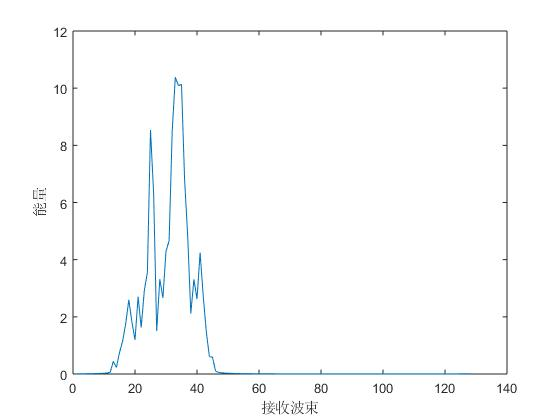
\includegraphics[width=0.6\textwidth]{img/2_2.jpg} \caption{用户单天线波束域信道能量耦合矩阵}
\end{figure}
多用户时,还可以发现,单个用户只占用部分波束,在一定情况下,可以将用户分配不同的波束,从而减少传输中不同用户的干扰,从而提高判断各用户的信号的准确度。
\begin{figure}[htbp!]
	\centering 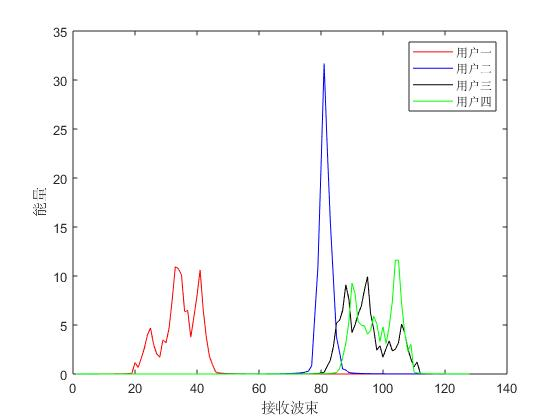
\includegraphics[width=0.6\textwidth]{img/2_5.jpg} \caption{多用户波束域信道能量耦合矩阵}
\end{figure}
考虑用户多天线的情况,此时耦合矩阵不再是单维的,所以多天线的耦合矩阵是3维视图
\begin{table}[htbp]
	\centering
	\caption{\label{tab:test}SCM仿真参数设置}
	\begin{tabular}{ll}
		\toprule
		参数 &  设置值 \\
		\bottomrule
		场景 &  郊区宏蜂窝 \\
		\bottomrule
		基站侧天线数 & 128 \\
		\bottomrule
		用户数天线	& 4 \\
		\bottomrule
		天线间距 & 0.5$\lambda$ \\
		\bottomrule
		路径数 & 6 \\
		\bottomrule
	\end{tabular}
\end{table}

\begin{figure}[htbp!]
	\centering 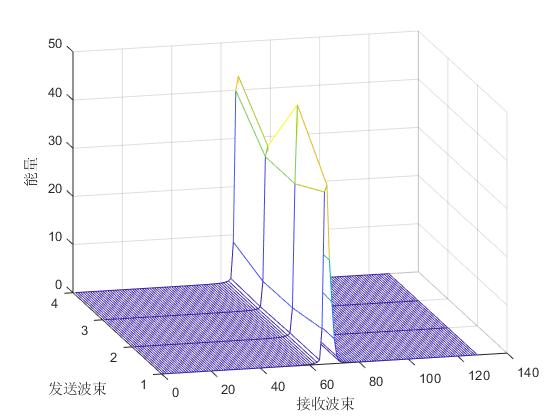
\includegraphics[width=0.6\textwidth]{img/2_3.jpg} \caption{用户多天线波束域信道能量耦合矩阵}
\end{figure}

由上面两图可以看出能量集中波束上,并且天线和AOA角对应同时也和波束对应。

\subsection{特征矩阵稀疏性}
本文上面也推导过相关阵的各元素表达式,上行信道,所以基站侧相关阵参考(2.22)
\begin{equation}\label{key}
\mathbf{R}_{F,r} = \mathbb{E} \lbrace \mathbf{H}_{F} (\mathbf{H}_{F})^{H} \rbrace
\end{equation}
则有相关阵的第(i,j)个元素为
\begin{eqnarray}\label{key}
[ \mathbf{R}_{F,r} ]_{i,j} & = &\mathbb{E} \lbrace \mathbf{h}_{F} (\mathbf{h}_{F})^{H} \rbrace  \nonumber \\
& = & \sum_{p=1}^{P} \sigma_{\beta_p}^{2} \mathbf{w}_{t}(\theta_{AOD}) \mathbf{w}_{t}^{H}(\theta_{AOD}) N_R \delta \left( 0.5\sin \theta_{AOA} - \frac{\tilde{i}-1}{N_R} , 0.5\sin \theta_{AOA} - \frac{\tilde{j}-1}{N_R} \right) \nonumber \\
\end{eqnarray}
由式(2.37)可知,当$ i \neq j$时, $ [ \mathbf{R}_{F,r} ]_{i,j} = 0$,即基站侧相关阵的为对角阵。由于基站侧相关阵为对角阵,并且存在有阵列响应矩阵在该位置较小或者为0,所以相关阵不一定满秩,且为对角阵,即利用相关阵计算可以利用对角阵的数学性质进行化简,并且因为其稀疏性质将大大减少MMSE的计算复杂度。通过验证波束域信道对应波束的SCM信道,同样通过相关阵的示意图,本文可以验证特征矩阵的稀疏性质。
考虑多天线多用户的情况,参数设置如下
\begin{table}[htbp]
	\centering
	\caption{\label{tab:test}SCM仿真参数设置}
	\begin{tabular}{ll}
		\toprule
		参数 &  设置值 \\
		\bottomrule
		场景 &  郊区宏蜂窝 \\
		\bottomrule
		基站侧天线数 & 128 \\
		\bottomrule
		用户数天线	& 4 \\
		\bottomrule
		天线间距 & 0.5$\lambda$ \\
		\bottomrule
		路径数 & 6 \\
		\bottomrule
	\end{tabular}
\end{table}
\begin{figure}[htbp!]
	\centering 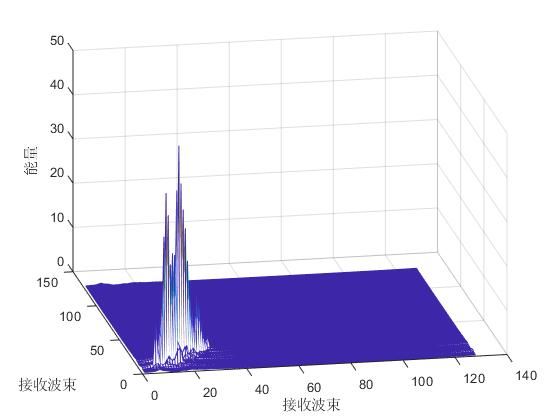
\includegraphics[width=0.6\textwidth]{img/2_4.jpg} \caption{用户多天线波束域信道基站侧相关阵}
\end{figure}

由上图,可以看出本文生成的信道模型的基站侧相关阵为对角阵,并且很多对角阵上的值为0或者很小可以不做考虑,所以利用特征矩阵计算MMSE检测算法将大大减少
检测时的计算复杂度。

\section{本章小结}
本章主要研究了MIMO信道物理模型,统计模型和波束域信道模型。其中物理模型主要是研究了影响信道情况的各种参数,并为后续各种模型的基础。统计信道模型主要研究了联合相关模型,作为实际相关仿真模型的基础模型。波束域信道模型主要体现的是大规模MIMO信道的特性和研究方式,通过波束域信道模型的特征,提供了减少计算复杂度切入点。

\chapter{基于MMSE接收机的复杂度优化}
\section{引言}
信号在通过上述复杂信道之后,信号会发生改变,此时需要利用一些判决方法将接收信号恢复为发送信号。但是因为通过信道后信号同样会收到随机干扰,所以完全恢复为初始信号某种意义上是不存在的,但是通过一些方法,可以尽可能地或者说最大概率的接近发送信号。这些根据接收信号恢复发送信号的方法在通信系统中称为检测,目前针对MIMO系统最佳的检测方法为MMSE估计。但是MMSE估计的计算复杂度随着天线的增多,信道矩阵维度的扩大,会变得非常高,实际系统实现会非常占用资源。而其主要复杂度主要来自于矩阵的求逆运算,而通过QR分解,可以将矩阵求逆运算化简为QR分解。QR分解的复杂度会比原始MMSE的复杂度大大降低。并且本文在信道模型重点描述了波束域信道,此时可以注意到波束域信道的信道是稀疏的,同样一定程度上减少了计算复杂度,本章的后续部分还会讨论空间域的MMSE以及复杂度优化
\section{系统模型}
在一个大规模MIMO系统中,一个基站将使用数以百计的天线来提供巨大的用户容量提高。在用户端,一般认为用户只有一根天线。但是,由于目前用户多天线的技术已经运用,将用户多天线应用到大规模MIMO系统中具有理论与实践的双重意义。所以在建立系统模型时,可以考虑用户多天线的情况。本文后续仿真将同时考虑用户单天线,用户多天线单流,用户多天线多流的情况。系统模型如下

考虑一个由一个基站(BS)和K个用户终端组成的系统,其中K个用户分别讨论其拥有单天线和多天线的情况。基站(BS)配有$N_R$根天线,第$k$个用户终端拥有$M_k$根天线,并且$\sum_{k=1}^K M_k = M$。根据上面的推导,可以得到基站第n根接收第i个用户的第r根的信号为
\begin{equation}\label{key}
r_{n,r} = \sum^{M_i}_{i=1} \sum_{p=1}^{P} \sum_{q=1}^{Q_p} \mathrm{Re} \left \lbrace u_{i,p,q} h_{p,q} (t) w_{i,p,q} s_b(t) e^{j 2\pi f_c t} \right \rbrace + n_{n,r}(t)
\end{equation}
其中,$h(t)$ 和 阵列响应如上。
\begin{eqnarray}\label{key}
h_{p,q}(t) = \alpha_{LNA}\beta\alpha_{PA}a_{p,q}e^{j(2\pi 
	(v_{p,q}t-v_{p,q}\tau_{p,q})+\phi_{p,q}
	)} \\
w_{n_{T},p,q} = \mathrm{exp}(-j2\pi \frac{d_{n_{T}}}{\lambda}\sin \theta_{p,q,AOD})\\
u_{n_{R},p,q} = \mathrm{exp}(-j2\pi \frac{d_{n_{R}}}{\lambda}\sin \theta_{p,q,AOA})
\end{eqnarray}
矩阵表达如下
\begin{eqnarray}\label{key}
\mathbf{r}_{i}(t) = [r_{1,i}(t) \quad r_{2,i}(t) \quad\dots\quad r_{N_{R},i}(t)]^{T} \\
\mathbf{s}_{i}(t) = [s_{1,i}(t) \quad s_{2,i}(t) \quad\dots\quad s_{N_{T},i}(t)]^{T} \\
\mathbf{n}_{i}(t) = [n_{1,i}(t) \quad n_{2,i}(t) \quad\dots\quad n_{N_{R},i}(t)]^{T} \\
\mathbf{H}_{i,p}(t) = \left[ \begin{array}{cccc}
h_{1,1,p}(t) & h_{1,2,p}(t) & \ldots & h_{1,M_{i},p}(t) \\
h_{2,1,p}(t) & h_{2,2,p}(t) & \ldots & h_{2,M_{i},p}(t) \\
\vdots & \vdots & \ddots & \vdots \\
h_{N_{R},1,p}(t) & h_{N_{R},2,p}(t) & \ldots & h_{N_{R},M_{i},p}(t)
\end{array} \right] 
\end{eqnarray}
由上面的矩阵表达和信号的物理表达式,可以将基带信号建模为
\begin{equation}\label{key}
\mathbf{r}_{i}(t) = \sum_{p=1}^{P}\mathbf{H}_{i,p}(t)s_{i}(t) + n_{i}(t)
\end{equation}
本文在这里将信道模型简写为
\begin{equation}\label{key}
\mathbf{y} = \sum_{i=1}^{K} \mathbf{H}_i \mathbf{x}_i + \mathbf{Z}
\end{equation}
有这样的性质
\begin{equation}\label{key}
\mathbb{E} \lbrace \mathrm{tr} (\mathbf{H}_i \mathbf{H}_i^H ) \rbrace = \frac{N M_i}{M}
\end{equation}
根据此性质$\mathbb{E} \lbrace \mathrm{tr} (\mathbf{H}_i \mathbf{H}_i^H ) \rbrace = \frac{N M_k}{M}$,本文可以套用联合相关信道模型
\begin{eqnarray}\label{key}
\mathbf{H}_i & = & \mathbf{U}_{r}\tilde{\mathbf{H}}\mathbf{U}_{t}^{H} = \mathbf{U}_{r}(\mathbf{D}+\mathbf{M}_i\odot \mathbf{H}_{idd})\mathbf{U}_{t}^{H} \\ \nonumber
& = & \mathbf{U}_{r}\mathbf{D}\mathbf{U}_{t}^{H} + \mathbf{U}_{r}(\mathbf{M}\odot \mathbf{H}_{idd})\mathbf{U}_{t}^{H}\mathbf{U}_{t}^{H}
\end{eqnarray}
其中$U_r$和$U_t$以及其他符号均与上面推导的式子相同,此处本文为了方便后续计算将$\mathbf{H}_{idd}$的方差设为$\frac{1}{M}$。
令
\begin{gather}\label{key}
\overline{\mathbf{H}}_i = \mathbf{U}_{r}\mathbf{D}\mathbf{U}_{t}^{H} \\
\tilde{\mathbf{H}}_i = \mathbf{U}_{r}(\mathbf{M}_i\odot \mathbf{H}_{idd})\mathbf{U}_{t}^{H}\mathbf{U}_{t}^{H}
\end{gather}
根据性质,可以得出结论
\begin{equation}\label{key}
\mathbb{E} \lbrace \tilde{\mathbf{H}}_i \mathbf{C}_{ij} \tilde{\mathbf{H}}_j^{H} \rbrace = 0_{N*N}
\end{equation}
\begin{equation}\label{key}
\mathbb{E} \lbrace \tilde{\mathbf{H}}_i^{H} \tilde{\mathbf{C}}_{ij} \tilde{\mathbf{H}}_j \rbrace = 0_{M_i*M_j}
\end{equation}
其中,$\mathbf{C}_{ij}$是一个$M_i \times M_j$ 维的常数矩阵,$\tilde{\mathbf{C}}_{ij}$ 是一个$N \times N$维的常数矩阵
类似上面统计信道,定义能量耦合矩阵为
\begin{equation}\label{key}
\bm{\Omega} =\mathbb{E}[\tilde{\mathbf{H}} \odot \tilde{\mathbf{H}}^{*}]
\end{equation}
即
\begin{equation}\label{key}
\bm{\Omega} =\mathbf{M_i} \odot \mathbf{M}
\end{equation}
则可以写出信道的单边相关矩阵$\tilde{\eta}_i$表达式
\begin{equation}\label{key}
\tilde{\eta}_i = \mathbb{E} \lbrace \tilde{\mathbf{H}}_i \mathbf{C}_i \tilde{\mathbf{H}}_i^H \rbrace
\end{equation}
根据上面的波束域模型推导和统计信道模型令矩阵$\tilde{\Pi}_i$为$N \times N$的对角矩阵
\begin{equation}\label{key}
\tilde{\Pi}_i = \sum_{j=1}^{M_i}[\Omega]_{ij}  [\mathbf{U}_t^H \mathbf{C}_i \mathbf{U}_t]_{jj}
\end{equation}
则有
\begin{equation}\label{key}
\tilde{\eta}_i = \mathbf{U}_r \tilde{\Pi}_i \mathbf{U}_r^H
\end{equation}
\section{MMSE接收机}
MMSE估计是最小均放误差估计的缩写,其判决准则如下式
\begin{equation}\label{key}
\hat{x}_{MMSE}(y) = \arg \min E[\| x - \hat{x} \|^{2}]
\end{equation}
根据期望的性质以及复矢量微分和复矩阵微分,要使误差最小对$\hat{x}^{*}$方向求梯度为0即可以得到
\begin{equation}\label{key}
\hat{x}_{MMSE}(y) = E[x|y]
\end{equation}
考虑线性最小均方误差,可以得出线性表达式
\begin{equation}\label{key}
\hat{x}_{LMMSE}(y)=Wy+b
\end{equation}
同一般情况的MMSE一致,线性最小均方误差是对$W^{*}$和$b^{*}$方向求梯度为0,以及设置在高斯白噪声信道下可以得到
\begin{equation}\label{key}
\left\{
\begin{array}{l}
W=C_{x}H^{H}(HC_{x}H^{H} + \sigma^{2}I)^{-1} \\
b=E[x] - C_{x}H^{H}(HC_{x}H^{H} + \sigma^{2}I)^{-1}HE[x]
\end{array}
\right.
\end{equation}
带入可得线性最小均方误差表达式
\begin{equation}\label{key}
\hat{x}_{LMSSE}(y)=E[x]+C_{x}H^{H}(HC_{x}H^{H}+\sigma^{2}I)^{-1}(y-HE[x])
\end{equation}
根据条件高斯PDF推导可得
\begin{equation}\label{key}
E{x|y}=\mu_{x}+C_{xy}C_{yy}^{-1}(y-E[y])
\end{equation}
\begin{equation}\label{key}
C_{x|y} = C_{xx} -C_{xy}C_{yy}^{-1}C_{yx}
\end{equation}
根据发送信号均值和接收信号均值,以及协方差矩阵可以得到
\begin{equation}\label{key}
E[x|y]=\mu_{x} + C_{x}H^{H}(HC_{x}H^{H}+\sigma^{2}I)^{-1}(y-H\mu_{x})
\end{equation}
\begin{equation}\label{key}
C_{x|y}=C_{x}-C_{x}H^{H}(HC_{x}H^{H}+\sigma^{2}I)^{-1}HC_{x}
\end{equation}
根据矩阵求逆定理
\begin{equation}\label{key}
(A + BCD)^{-1} = A^{-1} - A^{-1}B(DA^{-1}B+C^{-1})^{-1}DA^{-1}
\end{equation}
根据上式,可以将式(3.29)和(3.30)转换成如下形式
\begin{gather}\label{key}
E[x|y] = \mu_{x} + (HC_n^{-1}H^H + C_x^{-1})^{-1}H^H C_n^{-1}(y-H\mu_{x}) \\ 
C_{x|y} = (H C_n^{-1} H^H + C_x^{-1})^{-1}
\end{gather}
根据式(3.24)可以知道,且一般情况下,二进制采样后的信号均值为0,则MMSE的检测矩阵为
\begin{equation}\label{key}
{W} = ({H}{H}^H + \sigma^2 {I})^{-1}{H}^H
\end{equation}
同时得到MMSE准则计算公式
\begin{equation}\label{key}
\hat{x}_{MMSE} = (HH^H + \sigma^2 I)^{-1}H^H y
\end{equation}
而代入上述系统模型,则上式应写作
\begin{equation}\label{key}
\hat{\mathbf{x}}_{MMSE} = (\mathbf{H}\mathbf{H}^H + \sigma^2 \mathbf{I})^{-1}\mathbf{H}^H \mathbf{y}
\end{equation}
其中$\mathbf{H}$代表$[\mathbf{H}_1,\mathbf{H}_2,...,\mathbf{H}_K]$,令$\mathbf{x}$代表$[\mathbf{x}_1^T,\mathbf{x}_2^T,...,\mathbf{x}_K^T]$


根据MMSE估计,本文做了MMSE估计的仿真,并以MMSE估计作为评判基准,此处考虑的为BPSK调制。分别考虑用户单天线和用户多天线,多天线时设置为2
\begin{table}[htbp]
	\centering
	\caption{\label{tab:test}MMSE仿真参数设置}
	\begin{tabular}{ll}
		\toprule
		参数 &  设置值 \\
		\bottomrule
		场景 &  郊区宏蜂窝 \\
		\bottomrule
		基站侧天线数 & 128 \\
		\bottomrule
		用户数天线	& 1 \quad or\quad2 \\
		\bottomrule
		用户数	& 4 \\
		\bottomrule
		天线间距 & 0.5$\lambda$ \\
		\bottomrule
		路径数 & 6 \\
		\bottomrule
		用户采样数量 & 10000 \\
		\bottomrule
	\end{tabular}
\end{table}

\begin{figure}[htbp!]
	\centering 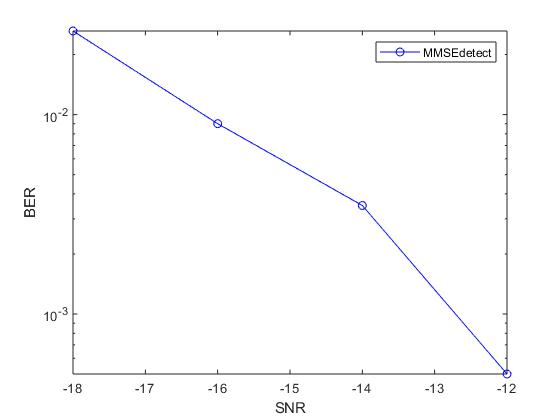
\includegraphics[width=0.45\textwidth]{img/3_1.jpg} \caption{单天线MMSE检测BER}
\end{figure}

\begin{figure}[htbp!]
	\centering 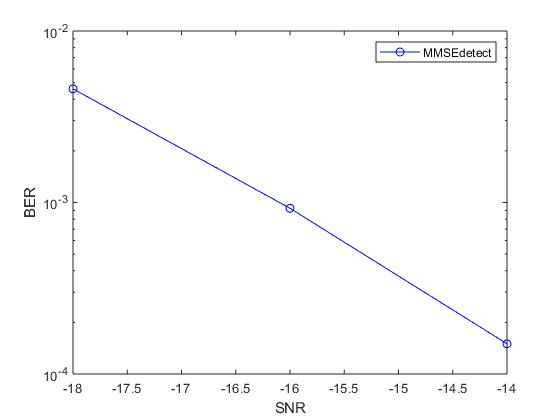
\includegraphics[width=0.45\textwidth]{img/3_3.jpg} \caption{多天线单流MMSE检测BER}
\end{figure}

\begin{figure}[htbp!]
	\centering 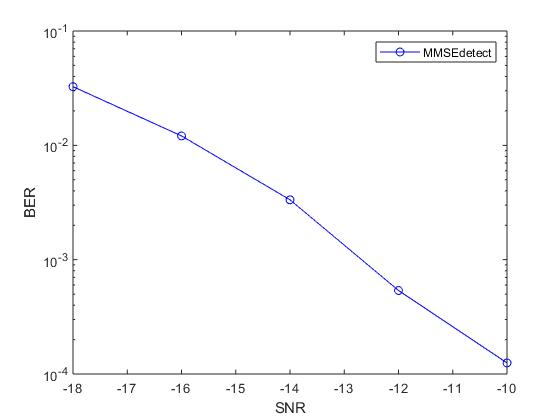
\includegraphics[width=0.45\textwidth]{img/3_8.jpg} \caption{多天线多流MMSE检测BER}
\end{figure}
从上图,可以看出对于不同的情况即用户单天线,用户多天线单流,用户多天线多流的情况各不相同。其中多天线单流应是判断准确度最高,其次为用户单天线,其次用户多天线多流。其中多天线单流,因为多天线传输的相同的数据能够通过综合所得到的数据得出最好的结果,而用户单天线与用户多天线多流的不同在于多天线多流带来了天线与天线之间的干扰,导致判断准确度下降。本文将主要从这三种情况对本文提出的低复杂度算法进行分析研究。而上述的MMSE模型将作为判断低复杂度算法是否达标的基准。

\section{QR分解}
虽然可以通过上式,很容易得到MMSE的检测矩阵的表达式,但需要注意的是信道矩阵$\mathbf{H}$是一个维度相对较大的矩阵,所以上式计算是非常困难的。并且在FPGA等硬件上实现矩阵求逆转置是比较繁琐的,所以通常MMSE矩阵硬件上实现是以QR分解为基础进行计算,其复杂度一定程度上得到简化。
下面简单介绍QR分解,即将信道矩阵分解为Q阵和R阵,其中Q阵为正交阵,R阵为上三角矩阵
令
\begin{equation}\label{key}
\overline{\mathbf{H}} = \left[
\begin{array}{c}
\mathbf{H}\\
\sigma \mathbf{I}
\end{array} \right] =
\left[
\begin{array}{c}
\mathbf{Q}_1\\
\mathbf{Q}_2
\end{array} \right] \mathbf{R}
\end{equation}
根据MMSE检测计算公式
\begin{equation}\label{key}
\hat{x}_{MMSE} = (\mathbf{H}\mathbf{H}^H + \sigma^2 \mathbf{I})^{-1}\mathbf{H}^H y
\end{equation}
有
\begin{equation}\label{key}
\mathbf{W}=(\overline{\mathbf{H}}^H \overline{\mathbf{H}})^{-1} \mathbf{H}^H
\end{equation}
\begin{equation}\label{key}
\mathbf{H} = \mathbf{Q}_1 \mathbf{R} ,\sigma\mathbf{I} = \mathbf{Q}_2\mathbf{R}
\end{equation}
又因为$\mathbf{Q}_1,\mathbf{Q}_2$是正交阵
\begin{equation}\label{key}
\mathbf{R} = \sigma \mathbf{Q}_2^{-1}
\end{equation}
\begin{equation}\label{key}
(\overline{\mathbf{H}}^H \overline{\mathbf{H}})^{-1} = (\mathbf{R}^H \mathbf{Q}^H\mathbf{Q} \mathbf{R})^{-1} =(\mathbf{R}^H \mathbf{R})^{-1}
\end{equation}
又有
\begin{equation}\label{key}
\mathbf{H}^{H} =\mathbf{R}^{H} \mathbf{Q}_1^H 
\end{equation}
所以式(3.39)有
\begin{equation}\label{key}
\mathbf{W} = \mathbf{R}^{-1} \mathbf{Q}_1^H
\end{equation}
由此可以容易得到检测矩阵的表达式为
\begin{equation}\label{key}
\mathbf{W}=(\overline{\mathbf{H}}^H \overline{\mathbf{H}})^{-1} \mathbf{H}^H = \frac{1}{\sigma} \mathbf{Q}_2 \mathbf{Q}_1^H
\end{equation}

下面本文简单介绍一下常用的QR分解的方法,一般使用QR分解可以用下面三种方法来完成,Gram-Schmit正交化QR分解,Givens矩阵与Givens旋转,householder矩阵与householder变换。上面三个不同的QR分解适合不同的系统模型,或者是指不同的情况下。
Gram-Schmit正交化适用于满秩矩阵,当$\mathbf{H}$为满秩矩阵时,$\overline{\mathbf{H}}$也是一个满秩矩阵。将$\overline{\mathbf{H}}$写为$[\alpha_1^T \alpha_2^T ... \alpha_n^T]$形式,
令
\begin{eqnarray}\label{key}
\beta_1 = \alpha_1 , \beta_2 = \alpha_2 - k\beta_1 , k = \frac{<\alpha_2,\beta_1>}{<\beta_1,\beta_1>} \nonumber
\end{eqnarray}
依次类推,则有
\begin{equation}\label{key}
\beta_i = \alpha_i - k_1\beta_1 -k_2\beta_2 - ... - k_{i-1}\beta_{i-1} \nonumber
\end{equation}
\begin{equation}\label{key}
k_j = \frac{<\alpha_i,\beta_j>}{<\beta_j,\beta_j>}, j= 1,2,3,...,i \nonumber
\end{equation}
从而,得到的$\mathbf{Q}$矩阵可令其为$[\beta_1^T,\beta_2^T,...,\beta_n^T]$,$\mathbf{Q}$矩阵是正交阵,$\mathbf{R}$矩阵是$\overline{\mathbf{H}}$到$\mathbf{R}$的变换矩阵。\\

Givens旋转主要是利用Givens矩阵的旋转特性去计算上三角阵$\mathbf{R}$而多个Givens矩阵的乘法和矩阵$\mathbf{G}_1...\mathbf{G}_n$根据Givens矩阵的特性也满足要求,为正交阵。
\begin{eqnarray}\label{key}
G(i,j,\theta) = \left[
\begin{array}{ccccccc}
1 & \ldots & 0 & \ldots & 0 & \ldots & 0 \\
\vdots & \ddots & \vdots & \quad & \vdots & \quad & \vdots \\
0 & \ldots & c & \ldots & s & \ldots & 0 \\
\vdots & \quad & \vdots & \ddots & \vdots & \quad & \vdots \\
0 & \ldots & -s & \ldots & c & \ldots & 0 \\
\vdots & \quad & \vdots & \quad & \vdots & \ddots & \vdots \\
0 & \ldots & 0 & \ldots & 0 & \ldots & 1 
\end{array}
\right]
\end{eqnarray}
$c=\cos\theta$ 和 $s = \sin\theta$ 出现在第i行和第j行与第i列和第j列的交叉点上,亦可以这样描述Givens矩阵的非零元素
\begin{gather}\label{key}
g_{kk} = 1 , \quad k \neq i,j  \nonumber\\ 
g_{ii} = c  \nonumber \\
g_{jj} = c  \nonumber \\
g_{ij} = s  \nonumber \\
g_{ji} = -s  \nonumber \\  
c=\cos\theta  \nonumber \\
s = \sin\theta  \nonumber
\end{gather}
主要是对目标矩阵的第i行和第j行进行变换。QR分解的Givens变换是为了将部分元素变换为0,即
\begin{eqnarray}\label{key}
\left[
\begin{array}{ccccccc}
1 & \ldots & 0 & \ldots & 0 & \ldots & 0 \\
\vdots & \ddots & \vdots & \quad & \vdots & \quad & \vdots \\
0 & \ldots & c & \ldots & s & \ldots & 0 \\
\vdots & \quad & \vdots & \ddots & \vdots & \quad & \vdots \\
0 & \ldots & -s & \ldots & c & \ldots & 0 \\
\vdots & \quad & \vdots & \quad & \vdots & \ddots & \vdots \\
0 & \ldots & 0 & \ldots & 0 & \ldots & 1 
\end{array}
\right]
\left[
\begin{array}{c}
x \\
\vdots \\
\alpha \\
\vdots \\
\beta \\
\vdots  \\
x
\end{array}
\right]
=\left[
\begin{array}{c}
x \\
\vdots \\
\gamma \\
\vdots \\
0 \\
\vdots  \\
x
\end{array}
\right]
\end{eqnarray}
即
\begin{equation}\label{key}
c = \frac{\alpha}{\sqrt{\alpha^2+\beta^2}}
\end{equation}
\begin{equation}\label{key}
s =\frac{\beta}{\sqrt{\alpha^2+\beta^2}}
\end{equation}
而类似(3.42),QR分解MMSE检测矩阵就是将$\mathbf{W}$看作列向量的结合,将向量按照从下至上依次转置为0,即
\begin{eqnarray}\label{key}
\left[
\begin{array}{cccccc}
1 & \ldots & 0 &  0 & \ldots & 0 \\
\vdots & \ddots & \vdots &  \vdots & \quad & \vdots \\
0 & \ldots & c &  s & \ldots & 0 \\
0 & \ldots & -s &  c & \ldots & 0 \\
\vdots & \quad & \vdots &  \vdots & \ddots & \vdots \\
0 & \ldots & 0 &  0 & \ldots & 1 
\end{array}
\right]
\left[
\begin{array}{ccc}
x_{11} & \ldots & x_{1n} \\
\vdots & \ldots & x_{pn}\\
\alpha & \ldots & x_{qn}\\
\beta& \ldots & x_{rn} \\
\vdots  & \ldots & x_{tn}\\
0& \ldots & x_{sn}
\end{array}
\right]
=\left[
\begin{array}{ccc}
x_{11}' & \ldots & x_{1n}'\\
\vdots & \ldots & x_{pn}'\\
\gamma & \ldots & x_{qn}'\\
0 & \ldots & x_{rn}'\\
\vdots  & \ldots & x_{tn}'\\
0& \ldots & x_{sn}'
\end{array}
\right]
\end{eqnarray}
通过$n*n/2$次Givens旋转,可以得到一个上三角阵,而Givens矩阵的乘积即为Q阵。\\

householder变换主要是利用householder矩阵将$\overline{\mathbf{H}}$特定位置的值转换为0,即求解$\overline{\mathbf{H}}$的上三角阵$\mathbf{R}$。householder矩阵对一个向量的表达式如下
\begin{equation}\label{key}
\mathbf{H} = \mathbf{I} - \frac{2}{<v,v>} v v^H
\end{equation}
即分别对$\overline{\mathbf{H}}$每列进行householder变化将其变换为上三角正,而householder矩阵的乘积和即为QR分解的$\mathbf{Q}$阵。
householder矩阵是对称矩阵,正交矩阵,hermitian矩阵,对合矩阵
\begin{gather}\label{key}
\mathbf{H}^T = \mathbf{H}  \nonumber \\
\mathbf{H}^T = \mathbf{H}^{-1}  \nonumber\\
\mathbf{H}^H = \mathbf{H}  \nonumber\\
\mathbf{H}^2 = \mathbf{I} \nonumber
\end{gather}
即可以根据$\mathbf{H}^H\mathbf{H}=\mathbf{I}$得到$vv^H =I$
而householder变换可以将矩阵变换到$v$向量代表的坐标轴的投影。即
\begin{equation}\label{key}
\mathbf{H}x =\alpha [1 \quad 0 \quad \ldots 0]^T
\end{equation}
令$e_1=[1 \quad 0 \quad \ldots 0]^T$,
根据householder矩阵的定义,可以得到
\begin{equation}\label{key}
\frac{1}{2}(x-\alpha e_1)=(v^Hx)v
\end{equation}
其中每一个$v$向量中的元素可以如下定义
\begin{eqnarray}\label{key}
v_1 & = & \frac{x_1-\alpha}{\| x - \alpha e_1 \|_2} \nonumber \\
& = & -\frac{\alpha-x_1}{\sqrt{2\alpha(\alpha-x_1)}} \nonumber \\
v_2 & = & \frac{x_2}{2\alpha v_1} \nonumber  \\
\vdots \nonumber \\
v_n & = & \frac{x_n}{2\alpha v_1}
\end{eqnarray}
利用householder变换求解QR分解的步骤大致如下,下面用$\mathbf{P}^{(n)}$表示第n个householder矩阵。目标矩阵写为
\begin{eqnarray}\label{key}
\mathbf{H}^{(i)} =
\left[
\begin{array}{ccccccc}
x_{11} & \ldots & x_{1i} & \ldots & x_{1j} & \ldots & x_{1k} \\
\vdots & \ddots & \vdots & \quad & \vdots & \quad & \vdots \\
0 & \ldots & x_{pi} & \ldots & x_{pj} & \ldots & x_{pk} \\
\vdots & \quad & \vdots & \ddots & \vdots & \quad & \vdots \\
0 & \ldots & x_{qi} & \ldots & x_{qj} & \ldots & x_{qk} \\
\vdots & \quad & \vdots & \quad & \vdots & \ddots & \vdots \\
0 & \ldots & x_{ni} & \ldots & x_{nj} & \ldots & x_{nk} 
\end{array}
\right]
\end{eqnarray}
对i列进行处理,即选取i列的$i+1 ~ n$个元素,用$S$代替,得到第i个householder矩阵$\mathbf{P}^{(i)}$,即
\begin{equation}\label{key}
\mathbf{P}^{(i)} \S = [1 \quad 0 \quad \ldots 0]^T
\end{equation}
即
\begin{equation}\label{key}
\mathbf{P}^{(i)}\mathbf{H}^{(i)} =\mathbf{P}^{(i)}
\left[
\begin{array}{ccccccc}
x_{11} & \ldots & x_{1i} & \ldots & x_{1j} & \ldots & x_{1k} \\
\vdots & \ddots & \vdots & \quad & \vdots & \quad & \vdots \\
0 & \ldots & x_{pi} & \ldots & x_{pj} & \ldots & x_{pk} \\
\vdots & \quad & \vdots & \ddots & \vdots & \quad & \vdots \\
0 & \ldots & x_{qi} & \ldots & x_{qj} & \ldots & x_{qk} \\
\vdots & \quad & \vdots & \quad & \vdots & \ddots & \vdots \\
0 & \ldots & x_{ni} & \ldots & x_{nj} & \ldots & x_{nk} 
\end{array}
\right]
= 
\left[
\begin{array}{ccccccc}
x_{11} & \ldots & x_{1i} & \ldots & x_{1j} & \ldots & x_{1k} \\
\vdots & \ddots & \vdots & \quad & \vdots & \quad & \vdots \\
0 & \ldots & x_{ii} & \ldots & x_{ij} & \ldots & x_{ik} \\
\vdots & \quad & \vdots & \ddots & \vdots & \quad & \vdots \\
0 & \ldots & 0 & \ldots & x_{qj} & \ldots & x_{qk} \\
\vdots & \quad & \vdots & \quad & \vdots & \ddots & \vdots \\
0 & \ldots & 0 & \ldots & x_{nj} & \ldots & x_{nk} 
\end{array}
\right]
\end{equation}
这个过程总共只需要进行n次即可以得到上三角阵$\mathbf{R}$,而变换矩阵的乘积即为正交矩阵$\mathbf{Q}$。

从本文上面所写的一般的MMSE复杂度主要是信道矩阵的求逆带来的,普通MMSE的复杂度为$Theta(M^3)$。如果采用QR分解优化的MMSE的计算,采用不同的QR分解有不同的复杂度。Gram-Schmit正交化QR分解和Givens变换QR分解的计算复杂度在计算一般信道矩阵时仍为$Theta(M^3)$。而householder变换的计算复杂度为$Theta(M^2)$。对于一般情况的信道矩阵时,Givens旋转计算复杂度并不会比普通的MMSE减少很多,但Givens旋转由于其矩阵的特定形式,可以只改变旋转的i行i列和j行j列,所以可以利用这个性质,对MMSE进行并行计算,从而降低MMSE检测的时间,但是计算复杂度上并不会减少。
由于QR分解计算MMSE是有严格数学推导的,所以所得到的结果应该与MMSE检测的结果一致。
\begin{figure}[htbp!]
	\centering 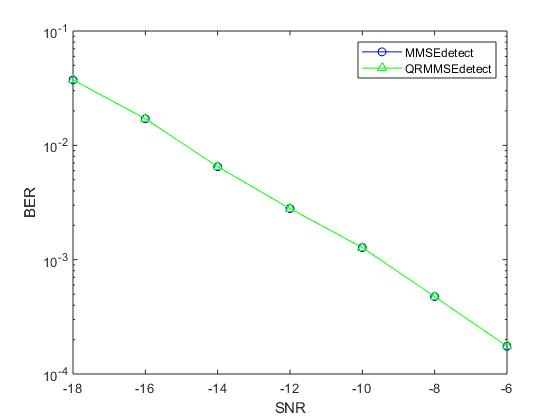
\includegraphics[width=0.45\textwidth]{img/3_9.jpg} \caption{QR分解MMSE}
\end{figure}

但是,可以注意到的是当矩阵稀疏时,Givens变换的计算复杂度就会降低。而推导QR分解使用矩阵
\begin{equation}\label{key}
\overline{\mathbf{H}} = \left[
\begin{array}{c}
\mathbf{H}\\
\sigma \mathbf{I}
\end{array} \right]
\end{equation}
其下半部分属于单位阵,所以在并行计算的同时,Givens变换的复杂度同样降低了n次操作,所以此时的Givens变换的计算复杂度同样为$\Theta(M^2)$
而由本文上面提到的波束域信道模型,当物理信道乘以信道矩阵的特征矩阵时,此时为波束域信道,信道矩阵为稀疏阵,此时使用Givens变换和householder变换的复杂度将会进一步的降低。但是在一般的信道矩阵,因为接收天线的数量不能逼近无穷大,按照一般公式无法计算出严格稀疏的信道矩阵,而讨论的降低复杂度需要稀疏矩阵。所以这里进行了近似处理,将相对较小的元素直接赋值为0。这必然会带来一定的误差,而接下来的部分,将利用仿真结果去判断。

\section{基于波束特性的MMSE接收机}
上部分提到了波束域信道相关阵是稀疏的,即某一个用户在基站接收侧时发射的信号能量在基站侧的某一些天线上得到了最大的能量,从而可以推知通过解耦



\chapter{基于PE接收机及复杂度优化}
\section{引言}
基于MMSE检测准则,利用检测矩阵约等式,利用系数代替检测矩阵,衍生出了PE接收机,即多项式展开(polynomial expansion)接收机。PE接收机其一定程度降低了复杂度,但是其不能很好的解决当上行信道用户天线总数比较大时系统检测矩阵系数计算仍然很复杂的问题。所以,本章节还会提出一种基于算子自由度的算法,将多项式展开得到的系数替换为确定性等同。通过替换可以略过计算多项式展开的计算,同时降低PE接收机的复杂度。本章将推导利用算子自由度理论证明算子自由等同能够代替系数,并且在一定程度上能够很好
\section{PE接收机}
通过上述计算过程,可以知道在用户数较多用户天线数较多的情况下,MMSE接收机的复杂度将会非常的高。所以基于MMSE接收机的基本原理有提出了多项式展开的方法对MMSE矩阵进行合理的化简,化简表达式如下
\begin{gather}\label{key}
\mathbf{W} = (\mathbf{H}\mathbf{H}^H + \sigma^2 \mathbf{I})^{-1}\mathbf{H}^H  \nonumber \\
\mathbf{x}_{MMSE} = \mathbf{W} \mathbf{y}  \nonumber \\
(\mathbf{H}^H\mathbf{H}+\sigma^2\mathbf{I})^{-1} \approx \sum_{i=1}^{L} b_{PE,i}^{(L)}(\mathbf{H}^H\mathbf{H})^{i-1}
\end{gather}
仍然利用MMSE接收机的判断准则
\begin{equation}\label{key}
\mathrm{arg} \min
\end{equation}
并令$\mathbf{b}^{(L)}_{PE}$ 表示 $b_{PE,i}^{(L)}$的合集。这里考虑的$L \leq M$,$M$为发送端用户天线总数
令
\begin{gather}\label{key}
\mathbf{B}_N = \mathbf{H}\mathbf{H}^H \nonumber \\
\mu_k = \frac{1}{N} \mathrm{tr}(\mathbf{B}_N^k) \nonumber
\end{gather}
其中$\frac{1}{N} \mathrm{tr}(\mathbf{B}_N^k)$指的是信道的经验矩。
\begin{gather}\label{key}
[\mathbf{\Phi}_{PE}]_{ij} = \mu_{i+j} + \sigma_{z}^2 \mu_{i+j-1} \nonumber \\
\left[\mathbf{\alpha}_{PE}\right]_i = \mu_i
\end{gather}

通过上式可以得到PE接收机检测表达式
\begin{equation}\label{key}
\hat{x}_{PE}^{(L)} = \sum_{i=1}^{L}b_{PE,i}^{(L)}(\mathbf{H}^H\mathbf{H})^{i-1}  \mathbf{H}^H y
\end{equation}
其中L的取值越大,计算复杂度越高,相对应的准确也会提升。
\begin{figure}[htbp!]
	\centering 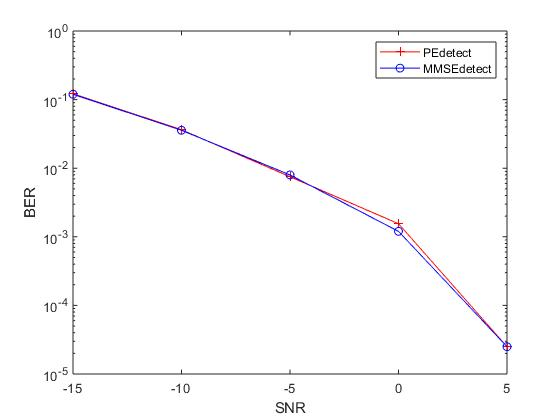
\includegraphics[width=0.6\textwidth]{img/3_2.jpg} \caption{L=3的普通PE接收机与MMSE接收机比较}
\end{figure}

\section{算子确定性等同替换}
上面为使用MMSE准则的多项式接收机,可以注意到当信道矩阵的维度较大的时候,利用经验矩计算每个信道同样会有较大的复杂度。但是在信道慢变的情况下,数据CSI变化得非常的慢,可以利用确定性等同$\overline{\mu}_k$代替$\mu_k$。此时,PE接收机只用计算$\sum_{i=1}^{L} b_{PE,i}^{(L)}(\mathbf{H}^H\mathbf{H})^{i-1}$ 即可。此式又可以被称为Krylov 域的计算,计算复杂度只有$\Theta(M^2)$。这里提出了利用算子自由度从而得到$\overline{\mu}_k$的方法。考虑本文是建立在大规模MIMO背景下的,所以本章开头提到的基站侧接收天线数量$N_R$可以看作是数量相当大。

所以参考文献,当$N \rightarrow \infty$,有$\mu - \mathbb{E}[\mu] \rightarrow 0$。写成公式
\begin{equation}\label{key}
\lim_{N \rightarrow \infty} \mathbb{E}[\mu_k] -\mu_k =0
\end{equation}
不过即使这步趋近并不能很好的获得,仍然可以利用下面的公式进行替代原来的方法。
\begin{gather}\label{key}
[\mathbf{\Phi}_{PE}]_{ij} = \mathbb{E}[\mu_{i+j}] + \sigma_{z}^2 \mathbb{E}[\mu_{i+j-1}] \nonumber \\
\left[\mathbf{\alpha}_{PE}\right]_i = \mathbb{E}[\mu_i]
\end{gather}
但是式(3.41)的请况并不在本文的考虑范围内,所以接下来本文将用$\mathbb{E}[\mu]$代替$\mu$。而本文提出的利用算子自由度,即将期望$\mathbb{E}[\mu]$由数转为算子,利用算子自由度对其进行计算。
这里本文简要介绍算子自由度的定义。

线性映射$E$是一个条件期望,如果其满足对于所有$b$,都有$E[b]=b$,对于所有$x$属于集合$\mathcal{A}$,$b_1,b_2$属于集合$\mathcal{B}$都有$E[b_1\mathcal{X}b_2]= b_1E[\mathcal{X}]b_2$。令$\mathcal{A}$表示酉代数,$\mathcal{B}$表示酉子代数,$E:\mathcal{A}->\mathcal{B}$是一个条件期望。则称$(\mathcal{A},E)$是$\mathcal{B}$算子值的自由空间。$\mathcal{B}$算子值概率空间元素成为$\mathcal{B}$算子值随机变量。$\mathcal{B}$算子值自由度乘法映射$\lbrace f_{\pi} \rbrace _{\pi \in NC(n)}:\mathcal{A}^n \rightarrow \mathcal{B}$
\begin{equation}\label{key}
f_{\pi_1 \bigsqcup \pi_2}^{\mathcal{B}}(\mathcal{X}_1,\mathcal{X}_2,...,\mathcal{X}_n) = f_{\pi_1}^{\mathcal{B}}(\mathcal{X}_1,\mathcal{X}_2,...,\mathcal{X}_n)f_{\pi_2}^{\mathcal{B}}(\mathcal{X}_1,\mathcal{X}_2,...,\mathcal{X}_n)
\end{equation}
$NC(n)$只n长度中不互相交叉的段,$\pi_1$和$\pi_2$就是其中的两个。

用$\mathcal{V}_{\pi}^{\mathcal{B}}(\mathcal{X}_1,\mathcal{X}_2,...,\mathcal{X}_n) = E((\mathcal{X}_1\mathcal{X}_2...\mathcal{X}_n))$定义$\mathcal{B}$算子值自由度乘法映射$\mathcal{V}_{\pi}^{\mathcal{B}} :\mathcal{A}^n \rightarrow \mathcal{B}$
。而算子的累差值同样也是算子自由度乘法映射可以由下式定义
\begin{equation}\label{key}
E((\mathcal{X}_1\mathcal{X}_2...\mathcal{X}_n)) = \sum_{\pi \in NC(n)} \mathcal{K}_{\pi}^{\mathcal{B}}(\mathcal{X}_1,\mathcal{X}_2,...,\mathcal{X}_n)
\end{equation}
则有
\begin{equation}\label{key}
\sum_{\pi \in NC(n)} \mathcal{K}_{\pi}^{\mathcal{B}}(\mathcal{X}_1,\mathcal{X}_2,...,\mathcal{X}_n) = \mathcal{V}_{\sigma}^{\mathcal{B}}(\mathcal{X}_1,\mathcal{X}_2,...,\mathcal{X}_n)\mu(\sigma,\pi)
\end{equation}
利用M\"{o}bius函数可以写为
\begin{equation}\label{key}
\mathcal{K}_{\pi}^{\mathcal{B}}(\mathcal{X}_1,\mathcal{X}_2,...,\mathcal{X}_n) = \sum_{\sigma<\pi, \in \pi \in NC(n)} \mathcal{V}_{\sigma}^{\mathcal{B}}(\mathcal{X}_1,\mathcal{X}_2,...,\mathcal{X}_n)\mu(\sigma,\pi)
\end{equation}
随机变量$\mathcal{X}$的$\mathcal{B}$算子R阶变换为
\begin{equation}\label{key}
\mathcal{R}_{\mathcal{X}}(b)=\sum_{n \geq 0} \mathcal{K}_{n+1}^{\mathcal{B}}(\mathcal{X}b,\mathcal{X}b,...,\mathcal{X}b,\mathcal{X}b,\mathcal{X})
\end{equation}
如有一个$\mathcal{B}$算子随机变量$\mathcal{X} \in \mathcal{A}$有
\begin{equation}\label{key}
\mathcal{R}_{\mathcal{X}}(b)=\mathcal{K}_2(\mathcal{X}b,\mathcal{X})
\end{equation}
则称其为$\mathcal{B}$算子半圆变量。

下文将主要介绍如何利用上面的公式得到$\overline{\mu}$的等同确定量。根据(3.13)(3.14)可以得到$\mathbf{H} = \overline{\mathbf{H}} + \tilde{\mathbf{H}}$
令
\begin{equation}\label{key}
\overline{\mathbf{X}} = \left(
\begin{array}{cc}
0_N & \overline{\mathbf{H}} \\
\overline{\mathbf{H}}^H & 0_M
\end{array}
\right)
\end{equation}
与
\begin{equation}\label{key}
\tilde{\mathbf{X}} = \left(
\begin{array}{cc}
0_N & \tilde{\mathbf{H}} \\
\tilde{\mathbf{H}}^H & 0_M
\end{array}
\right)
\end{equation}
并令$\mathbf{X} = \tilde{\mathbf{X}} + \overline{\mathbf{X}}$,$\tilde{\mathbf{W}}_k$代表$\mathbf{M}_k \odot \mathbf{W}_k$,$\eta(\mathbf{D})$代表$\mathbb{E}\lbrace \tilde{\mathbf{X}} \mathbf{D} \tilde{\mathbf{X}} \rbrace $ 。 根据信道模型,可以得到$\mathbb{E}[\mu_k]$与$\mathbf{X}$的矩有关。
又有
\begin{equation}\label{key}
\mathbf{X}^2 = \left(
\begin{array}{cc}
\mathbf{H}\mathbf{H}^H & 0_{N*M} \\
0_{M*N} & \mathbf{H}^H\mathbf{H}
\end{array}
\right)
\end{equation}
又令
\begin{equation}\label{key}
\tilde{\mathbf{X}}_k = 
\left(
\begin{array}{cc}
0_N & \hat{\mathbf{H}}_k \\
\hat{\mathbf{H}}^H_k & 0_M
\end{array}
\right)
\end{equation}
其中$\hat{\mathbf{H}}_k$代表$[ 0_{N*M_1} \ldots \tilde{\mathbf{H}}_k \quad 0_{N*M_{k+1}} \ldots]$,所以有下式
\begin{equation}\label{key}
\tilde{\mathbf{X}} = \sum_{k=1}^{K} \tilde{\mathbf{X}}_k
\end{equation}
根据上面信道模型,可以写出$\tilde{\mathbf{H}}_k = \mathbf{U}_k \tilde{\mathbf{W}}_k \mathbf{V}_k^H$,同时可以改写$\tilde{\mathbf{X}}$
\begin{equation}\label{key}
\tilde{\mathbf{X}}_k = \mathbf{A}_k \hat{\mathbf{W}} \mathbf{A}^H
\end{equation}
其中$\hat{\mathbf{W}}$可以用下式表示
\begin{equation}\label{key}
\left(
\begin{array}{ccccc}
0_N & \ldots & \tilde{\mathbf{W}} & 0_{N*M_{k+1}} & \ldots \\
\vdots & \ddots & \ldots & \ldots & \ldots \\
\tilde{\mathbf{W}}^H & \ldots & 0_{M_k * M_k} & 0_{M_k*M_{k+1}} & \ldots \\
0_{M_{k+1}*N} & \ldots & 0_{M_{k+1} *M_k} & 0_{M_{k+1}*M_{k+1}} & \ldots \\
\vdots & \ldots & \vdots & \vdots & \ddots
\end{array}
\right)
\end{equation}
\begin{equation}\label{key}
\mathbf{A}_k = \mathrm{diag}(\mathbf{U}_k,0_{M_1},\ldots,\mathbf{V}_k,0_{M_{k+1}},\ldots)
\end{equation}

通过替换$\hat{\mathbf{W}}$中的独立高斯变变量为相同方差的自由圆形变量,可以获得自由确定性等同$\hat{\mathcal{W}}$。而此时,令$\hat{\mathcal{X}}_k = \mathbf{A}_k \hat{\mathcal{W}}_k \mathbf{A}_k$ 则也可以用自由确定性等同$\mathcal{X}$代替$\mathbf{X}$。一般的,自由确定性等同$\mathcal{X}$和原始模型数据$\mathbf{X}$在L趋近于无穷时都有相同算子分布。令$\mathcal{B}_N$代表$<\mathcal{X}>_N$。$<\mathcal{X}>_N$指的是$\mathcal{X}$行列下标1到N的子矩阵。
令$F_{\mathbf{B}_N}(\lambda)$代表随机矩阵$\mathbf{B}_N$的元素的累计分布。令$\mathbb{C}^+$代表集合$\lbrace z\in \mathbb{C}: \mathcal{J}(z) > 0 \rbrace$。参考文献,$z \in \mathbb{C}^+$的柯西变换$G_{\mathbf{B}_N}(z)$
\begin{equation}\label{key}
G_{\mathbf{B}_N}(z) = \int_0^\infty \frac{1}{z-\lambda} dF_{\mathbf{B}_N}(\lambda) = \frac{1}{N} \mathbb{E}\lbrace \mathrm{tr}(z \mathbf{I}_N - \mathbf{B}_N)^{-1}\rbrace
\end{equation}
对于所有代表柯西变换的$F_{\mathbf{B}_N}$,都有反变换,可以写成下面形式
\begin{equation}\label{key}
F_{\mathbf{B}_N}(\lambda) = -\frac{1}{\pi} \lim_{\epsilon \rightarrow 0^+} \int_{-\infty}^{\lambda}  \mathcal{J}(\mathbf{G}_{\mathbf{B}_N}(x+i\epsilon))dx
\end{equation}
参考文献,有柯西变换$G_{\mathcal{B}_N}(z)$是$G_{\mathbf{B}_N}(z)$的确定性等同
\begin{equation}\label{key}
\lim_{N \rightarrow \infty}(G_{\mathbf{B}_N}(z)-G_{\mathcal{B}_N}(z)) = 0
\end{equation}
$\mathcal{B}_N$是$\mathbf{B}_N$的确定性等同。并且有这样$\overline{\mu}_k = \frac{1}{N}\mathbb{E}[\mathrm{tr}(\mathcal{B}_N^k)]$。并且可作出这样的近似
\begin{equation}\label{key}
\lim_{N \rightarrow \infty} \mathbb{E}[\mu_k] -\overline{\mu_k} =0
\end{equation}
参考文献,给出的$E{\mu_m}$和$\mu_m$做比较
\begin{figure}[htbp!]
	\centering 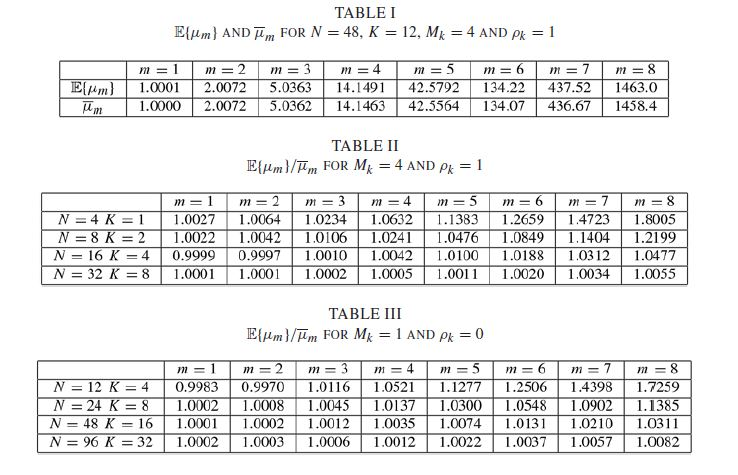
\includegraphics[width=1\textwidth]{img/3_6.jpg} 
\end{figure}

将原始模型的矩阵矩的确定性等同转换到算子自由度模型上。接着可以利用上文提到的算子自由度的定理和公式来计算$\overline{\mu}_k$。下文简要介绍计算理论,令$\mathcal{B}$表示代数$\mathcal{M}_{N+M}(\mathbb{C})$。利用元素的累差可以就计算出$\tilde{\mathcal{X}}_1,\tilde{\mathcal{X}}_2,\ldots,\tilde{\mathcal{X}}_K$。通过计算,可以得到所有的$\mathcal{B}$累差各不相同,并且只有第二阶$\mathcal{B}$算子累差是非零矩阵。因此$\tilde{\mathcal{X}}_1,\tilde{\mathcal{X}}_2,\ldots,\tilde{\mathcal{X}}_K$关于$\mathcal{B}$自由,并且每一个$\tilde{\mathcal{X}}$都是关于$\mathcal{B}$的半圆形变量。并且非零的累差可以用下式表示
\begin{equation}\label{key}
\mathcal{K}_2(\tilde{\mathcal{X}},\mathbf{D}\tilde{\mathcal{X}})=\mathbb{E}[\mathcal{X}\mathbf{D}\tilde{\mathcal{X}}]
\end{equation}
又因为上文所做的自由确定等同与原始模型的对应,还可以得到下式
\begin{equation}\label{key}
\mathbb{E}[\mathcal{X}\mathbf{D}\tilde{\mathcal{X}}]=
\mathbb{E}[\mathbf{X}\mathbf{D}\tilde{\mathbf{X}}] = \eta(\mathbf{D})
\end{equation}
同时,所有的高阶$\mathcal{B}$算子累差都是零矩阵。所以有下式表示一阶$\mathcal{B}$算子累差
\begin{equation}\label{key}
\mathcal{K}_2(\overline{\mathbf{X}}) = \overline{\mathbf{X}}
\end{equation}
之前有$\mathcal{X}=\overline{\mathbf{X}}+\tilde{\mathcal{X}}$因为$\overline{\mathbf{X}}\in \mathcal{B}$,本文$\overline{\mathbf{X}}$和$\overline{\mathcal{X}}$关于$\mathcal{B}$算子自由。
则有
\begin{gather}\label{key}
\mathcal{K}_1(\mathcal{X}) = \mathcal{K}_1(\overline{\mathbf{X}}) + \mathcal{K}_1(\overline{\mathcal{X}}) = \overline{\mathbf{X}} \nonumber\\
\mathcal{K}_2({\mathcal{X}},\mathbf{D}{\mathcal{X}})=\mathcal{K}_2(\tilde{\mathcal{X}},\mathbf{D}\tilde{\mathcal{X}}) + \mathcal{K}_2(\overline{\mathcal{X}},\mathbf{D}\overline{\mathcal{X}})\\ =\mathbb{E}[\mathcal{X}\mathbf{D}\tilde{\mathcal{X}}]\nonumber = 
\mathbb{E}[\mathbf{X}\mathbf{D}\tilde{\mathbf{X}}] = \eta(\mathbf{D})
\end{gather}
由此本文得到下面的推论来计算$\mathbb{E}[\mathcal{X}^k]$从而能够推导到$\overline{\mu}_k$。下面的递推公式可以计算出$\mathbb{E}[\mathcal{X}^k]$。
\begin{eqnarray}\label{key}
\mathbb{E}[\mathcal{X}^{2m+2}]=\overline{\mathbf{X}}\mathbb{E}[\mathcal{X}^{2m+1}]+\sum_{j=0}^{m}\eta(\mathbb{E}[\mathcal{X}^{2j}])\mathbb{E}[\mathcal{X}^{2m-2j}]  \\
\mathbb{E}[\mathcal{X}^{2m+1}]=\overline{\mathbf{X}}\mathbb{E}[\mathcal{X}^{2m}]+\sum_{j=0}^{m}\eta(\mathbb{E}[\mathcal{X}^{2j}])\mathbb{E}[\mathcal{X}^{2m-2j-1}] 
\end{eqnarray}
其中m是自然数,$\mathbb{E}[\mathcal{X}^0] = \mathbf{I}_n$

用代数形式表示$\mathcal{D}$
\begin{equation}\label{key}
\mathcal{D} = \mathrm{diag}(\mathcal{M}_N(\mathbb{C}),\mathcal{M}_{M_1}(\mathbb{C}),...,\mathcal{M}_{M_K}(\mathbb{C}))
\end{equation}
本文在论文模型部分讨论过所选用统计模型
\begin{equation}\label{key}
\mathbf{H} = \mathbf{U}_{r}\tilde{\mathbf{H}}\mathbf{U}_{t}^{H} = \mathbf{U}_{r}(\mathbf{D}+\mathbf{M}\odot \mathbf{H}_{idd})\mathbf{U}_{t}^{H}
\end{equation}
考虑其中的$\mathbf{D}$为0,在此算子自由度模型中即$\overline{\mathbf{X}} = 0_N$。即又可以得到下式的递推结论。
\begin{gather}\label{key}
\mathbb{E}[\mathcal{B}^{m+1}_N] = \sum_{j=0}^{m}(\sum_{k=0}^{K}\tilde{\eta_k}(\mathbf{S}_{jk}))\mathbb{E}[\mathcal{B}_N^{m-j}] \\
\mathbf{S}_{(m+1)k} =\sum_{j=0}^{m}\eta(\mathbb{E}(\mathcal{B}_N^j))\mathbf{S}_{m-j}k
\end{gather}
其中m是自然数,$\mathbb{E}[\mathcal{B}_N^0]=\mathbf{I}_N$和$\mathbf{S}_{0k}=\mathbf{I}_{M_k}$

以上是基于算子自由度低复杂度,下面将简要介绍低复杂多项式展开(PE)接收机的算法。如上文所叙述的,本文考虑的是$\overline{\mathbf{X}} = 0_N$的情况,所以低复杂度PE接收机首先根据式(3.66) 
和(3.67)计算$\mathbb{E}[\mathcal{B}_N^{m}]$和$\mathbf{S}_{(m)k}$。
\begin{equation}\label{key}
\overline{\mu}_{m} = \frac{1}{N} \mathrm{tr}(\mathbb{E}[\mathcal{B}_N^{m}])
\end{equation}
令维度为$L*L$的矩阵$\overline{\Phi}_{PE}$为
\begin{equation}\label{key}
[\overline{\Phi_{PE}}]_{ij} = \overline{\mu}_{i+j} + \sigma_z^2 \overline{\mu}_{i+j-1}
\end{equation}
令向量$\bm{\alpha}_{PE}$为
\begin{equation}\label{key}
[\overline{\bm{\alpha}}_{PE}]_i = \overline{\mu}_i
\end{equation}
利用上面两等式计算出估计系数为
\begin{equation}\label{key}
\overline{\mathbf{b}}_{PE}^{L} = \overline{\Phi}_{PE}^{-1} [\overline{\bm{\alpha}}_{PE}]
\end{equation}
带入系数PE接收机判决公式
\begin{equation}\label{key}
\hat{x}_{LPE}^{(L)} = \sum_{i=1}^{L}\overline{b}_{PE,i}^{(L)}(\mathbf{H}^H\mathbf{H})^{i-1}  \mathbf{H}^H y
\end{equation}

上面描述低复杂度PE接收机利用确定性等同进行计算,因为省略了计算多项式展开的系数的过程,那么用确定量计算的PE接收机计算复杂度将仅仅是Krylov域的计算,其计算复杂度为$\Theta(M^2)$,M为用户天线总数。

\section{基于算子}
上述给出的图形都是用户单天线的情况,可以看出在单天线条件下,L=3时,普通PE接收机和低复杂度PE接收机性能和MMSE接收机的性能是非常接近的。
下面将给出不同阶数的PE接收机和低复杂度PE接收机的性能图

用户天线为1,采样样本为4*10000
\begin{figure}[htbp!]
	\centering 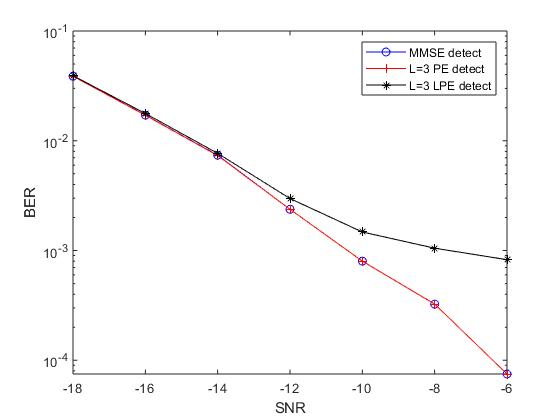
\includegraphics[width=0.6\textwidth]{img/3_5.jpg} \caption{单天线情况下 普通PE接收机,低复杂度PE接收机与MMSE接收机比较}
\end{figure}

\begin{figure}[htbp!]
	\centering 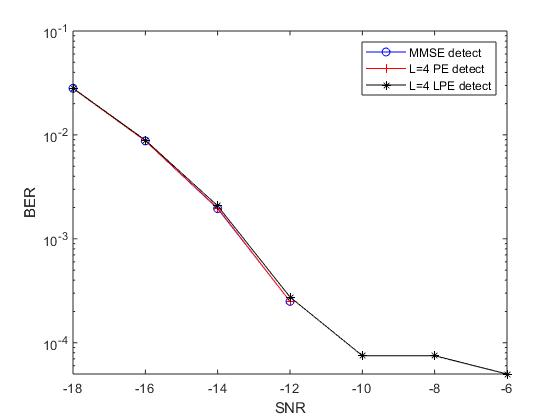
\includegraphics[width=0.6\textwidth]{img/3_7.jpg} \caption{单天线情况下 普通PE接收机,低复杂度PE接收机与MMSE接收机比较}
\end{figure}
从图4.3可以看出当阶数为4时,低复杂度PE接收机已经可以逼近MMSE接收机的性能。而在L<4的时候,低复杂度PE接收机的性能与一般的MMSE的接收机性能上还是有一些差距的。

PE接收机的性能随着阶数的增高会随之提升,本文将不再论证,下面主要讨论不同天线情况下低复杂度PE接收机的性能。




\end{Main} % 结束正文

%\begin{Acknowledgement}{}

%\end{Acknowledgement}

% 参考文献
%\bibliography{seuthesis}



\newpage
\printindex % 索引

%\begin{thebibliography}{99}


%\bibliographystyle{ieee}
%\bibliography{seuthesis}

 
\end{document}
